\chapter{Statistical Analysis and Results}\label{cha:fit}

In this chapter the likelihood fit is introduced, which is used to determine the signal strength of the $\Httllfull$ process.
For the multivariate analysis (MVA) the shape of the BDT output is used as the final discriminant.
In the cut-based analysis (CBA) the $\mmc$ distribution is used.
Furthermore, a strategy to obtain an optimal binning for the distribution of the BDT output is discussed.
Finally, the fit results are presented and compared between MVA and CBA\@.

\section{Likelihood fit}

The likelihood fit is used to determine the signal strength $\mu$, which is the ratio of the measured (fitted) signal cross-section to the
Standard Model prediction for cross-section times branching ratio of $\Httll$.
A value of $\mu = 0$ indicates the absence of signal, $\mu = 1$ corresponds to the case that the amount of signal matches with the SM prediction.
The fit is executed with the \texttt{HistFactory} tool~\cite{HistFactory} using the \texttt{RooStats}~\cite{RooStats} package and the \texttt{WSMaker}~\cite{WSMaker} script collection.

The fit is based on a binned likelihood function $\mathcal{L}$~\cite{FitATLAS}, which originates from the Poisson distribution,
\begin{equation}
    \mathcal{L}(\mu, \bm{\theta}) = \prod_{i=1}^{N_\text{bins}} = \frac{{\left(\mu s_i (\bm{\theta}) + b_i(\bm{\theta})\right)}^{n_i} e^{-(\mu s_i (\bm{\theta}) + b_i(\bm{\theta}))}}{n_i!} \,.
\end{equation}
The binned likelihood function gives the probability of finding $n$ data events in the bin $i$, where $s$ signal events and $b$ background events are expected.
Here, the bins are not limited to one observable, but different contributions, for example single bin categories and binned distributions, can be combined in the likelihood.
Additionally, the likelihood function depends on several nuisance parameters, $\bm{\theta} = (\theta_1, \ldots, \theta_m)$, which are discussed below.
A large value of the likelihood function indicates a better agreement between prediction and data.

The best fit value for $\mu$ is obtained by maximizing the likelihood function, and is denoted as $\hat{\mu}$.
However, it is more convenient to minimize the negative logarithm of the likelihood function, $- \ln \mathcal{L}$, which is also known as the negative log-likelihood (NLL).

In the search of new physics the compatibility between the observed data and the background-only hypothesis is an important quantity.
Therefore, the null hypothesis is $\mu = 0$ which needs to be rejected for an observation of the signal process.

First, a test statistic $q_0$ is constructed~\cite{FitATLAS},
\begin{equation}
    q_0 =
    \begin{cases}
        -2 \ln (\mathcal{L}(0, \hat{\hat{\bm{\theta}}}) / \mathcal{L}(\hat{\mu}, \hat{\theta})) & \hat{\mu} \geq 0 \\
        0 &  \hat{\mu} < 0
    \end{cases} \,,
\end{equation}
where $\mathcal{L}(\hat{\mu}, \hat{\theta})$ refers to the maximum of the likelihood function and $\mathcal{L}(0, \hat{\hat{\bm{\theta}}})$ to
an conditional maximum where $\mu$ is fixed according to the null hypothesis.
The test statistic should have a good separation between the null hypothesis and the alternative hypothesis, where the signal strength is non-vanishing.
If a negative amount of signal events is observed ($\hat{\mu} < 0$), which is unphysical, the test statistic is set to zero, since a positive amount is expected.
Using the probability density function of the test statistic, $g(q_0 | 0, \hat{\hat{\bm{\theta}}})$,
the compatibility of the null hypothesis with the observed test statistic $q_{0,\text{obs}}$
can be calculated, which is expressed with the $p_0$ value,
\begin{equation}
    p_0 = \int_{q_0,\text{obs}}^{\infty} g(q_0 | 0, \hat{\hat{\bm{\theta}}}) \dif q_0 \,.
\end{equation}
The $p_0$ value is the probability that the test statistic $q_{0}$
is at least as incompatible with the null hypothesis (here:\ background only) as the observed one, assuming that the background only
hypothesis is realized in nature.

Usually the $p_0$-value is expressed in terms of Gaussian standard deviations.
This is the so-called \emph{significance} $Z_0$, which can be calculated by
\begin{equation}
    \label{eq:fit:significance}
    Z_0 = \Phi^{-1} (1 - p_0) \simeq \sqrt{q_0} \,.
\end{equation}
Here, $\Phi$ is the cumulative distribution function of the Gaussian distribution.
The asymptotic approximation~\cite{FitATLAS} is used in \cref{eq:fit:significance} to simplify the calculation.

An observation is claimed for a $p_0$-value of $p_0 < \num{2.85e-7}$, which corresponds to a significance of $Z_0 \geq 5$.

\section{Fitting Procedure}\label{sec:fit:procedure}

For the construction of the likelihood function several signal and control regions are used, which are discussed below.

In the cut-based analysis four signal regions, two for the VBF category and two for the boosted category as explained in \cref{sec:event_selection:categorization} is used.
The binning is setup in such a ways that there is at least some amount of background in each bin.
Under and overflow bins are included in the first and last bin, respectively.

An overview of the binning is given in \cref{tab:fit:regions:cba}.
To obtain the normalization of the $\Zll$and top-background a dedicated control region is used for each background.
There are separate control regions for the VBF and boosted category.
The definitions of the control regions can be found in \cref{sec:background_estimation:normalization}.
Since the control regions are used only for normalization purposes, only a single bin is used, which contains the complete event count.

\begin{table}[htpb]
    \centering
    \caption{Overview of the binning in the signal regions (SR) and control regions (CR) used in the fit for the cut-based analysis.}\label{tab:fit:regions:cba}
    \begin{tabular}{lcc}
        \toprule
        Region                              & Type  & Binning [GeV] \\ \midrule
        high VBF                            & SR    & $\left[60, 88, 116, 130, 200\right]$ \\
        low VBF                             & SR    & $\left[60, 88, 116, 130, 200\right]$ \\
        high boosted                        & SR    & $\left[60, 80, 110, 120, 130, 140, 200\right]$ \\
        low boosted                         & SR    & $\left[60, 80, 110, 120, 130, 140, 200\right]$ \\
        $\Zll$ VBF control region (CBA)     & CR    & single bin\\
        Top VBF control region (CBA)        & CR    & single bin\\
        $\Zll$ boosted control region (CBA) & CR    & single bin\\
        Top boosted control region (CBA)    & CR    & single bin\\
    \end{tabular}
\end{table}

In the multivariate analysis a similar approach is applied.
For the signal regions distributions of the BDT output after the modified event selection (\cref{sec:mva:event_selection}) are used.
In the boosted category the individual BDTs for same flavour (SF) and different flavour (DF) events are taken.
However, it turned out that splitting the events into SF and DF in the VBF category actually decreased the significance, because
insufficient amount of statistics.
Therefore, the BDTs for SF and DF events are combined by adding up the event yields in the individual bins.
The control regions are based on the modified event selection, but no other changes were made.

The binning for the BDT distributions is calculated with a method similar to the one used
in the Run-1 analysis of the $\Httlh$ channel~\cite{RuthmannPhd}.
Most signal events can be found at higher values of the BDT output distribution, whereas most background events
are located at low values.
A fine binning would allow for a better measurement of the signal strength, since bins in the region of high BDT values
would contain only a small number of background events.
However, each bin must contain at least some amount of background events to ensure that statistical fluctuations of the
background do not lead to empty bins.
The following algorithm provides the finest binning possible without violating the robustness of the background estimation.
A fine binned BDT distribution with 200 bins is used as an input.

Starting from the very signal like end of the BDT distribution the bins are merged if all of the following criteria are met:
\begin{itemize}
    \item The expected yield of the total background has to be larger than the expected yield of total background events in the current bin.
    \item The relative statistical uncertainty of each background ($\Zll$, $\Ztautau$, diboson, top, fake, $H \to WW$) has to be smaller than \SI{100}{\percent}.
    \item Either the expected yield yield of the total background is \SI{50}{\percent} larger than in the previous bin or
        the signal-to-background ratio is at most \SI{10}{\percent} smaller than in the previous bin.
\end{itemize}

The first criterion ensures a background shape which is monotonically decreasing.
Due to the second criterion it is ensured that statistical fluctuations of the background do not lead to empty bins.
The third criterion is used to create a new bin, if the bin offers higher signal sensitivity or if the background composition
is much different than in the previous bin.

The algorithm is applied on the BDTs for SF and DF events in the boosted category and on the combined BDT in the VBF category.
An overview of the different regions and binnings used in the multivariate analysis is shown in \cref{tab:fit:regions:mva}.

\begin{sidewaystable}[htpb]
    \centering
    \caption{Overview of the binning in the signal regions (SR) and control regions (CR) used in the fit for the multivariate analysis.}\label{tab:fit:regions:mva}
    \begin{tabular}{lcc}
        \toprule
        Region                              & Type  & Binning \\ \midrule
        VBF                                 & SR    & $\left[-1, -0.47, -0.24,  0.19, 0.59, 0.74, 1\right]$ \\
        Boosted SF                          & SR    & $\left[-1, -0.78, -0.44, -0.19, 0.12, 0.29, 0.41, 0.49, 0.57, 0.64, 0.69, 0.72, 1\right]$ \\
        Boosted DF                          & SR    & $\left[-1, -0.78, -0.5,  -0.21, 0.1,  0.31, 0.42, 0.5,  0.57, 0.61, 0.65, 0.67, 0.69, 1\right]$ \\
        $\Zll$ VBF control region (MVA)     & CR    & single bin\\
        Top VBF control region (MVA)        & CR    & single bin\\
        $\Zll$ boosted control region (MVA) & CR    & single bin\\
        Top boosted control region (MVA)    & CR    & single bin\\
    \end{tabular}
\end{sidewaystable}

\section{Results}\label{sec:fit:results}

The likelihood fit is carried out for both the cut-based and multivariate analysis.
Because this analysis is still under development and not yet approved by the ATLAS collaboration, the fit cannot be done
with the observed data.
Instead, the so-called \emph{Asimov data}~\cite{FitATLAS} are used, where the simulated events act as an replacement for the observed data.
Therefore, the extracted signal strength will always be one.
But the fit can still be used to obtain an expected sensitivity and to validate the fitting procedure.
The distributions of $\mmc$ which are used in the fit of the CBA are shown in \cref{fig:fit:input:cba:SR,fig:fit:input:cba:CR}, whereas the
corresponding distributions of the BDT output for the MVA are shown in \cref{fig:fit:input:mva:SR,fig:fit:input:mva:CR}.
As can be seen the control regions are relatively pure in their respectively processes, see also \cref{sec:background_estimation:normalization}.
The contributions of the ``fake'' background in the $\Zll$ control regions are minimal and therefore neglected.

\begin{figure}[htb]
    \centering
    \begin{subfigure}[t]{0.45\textwidth}
        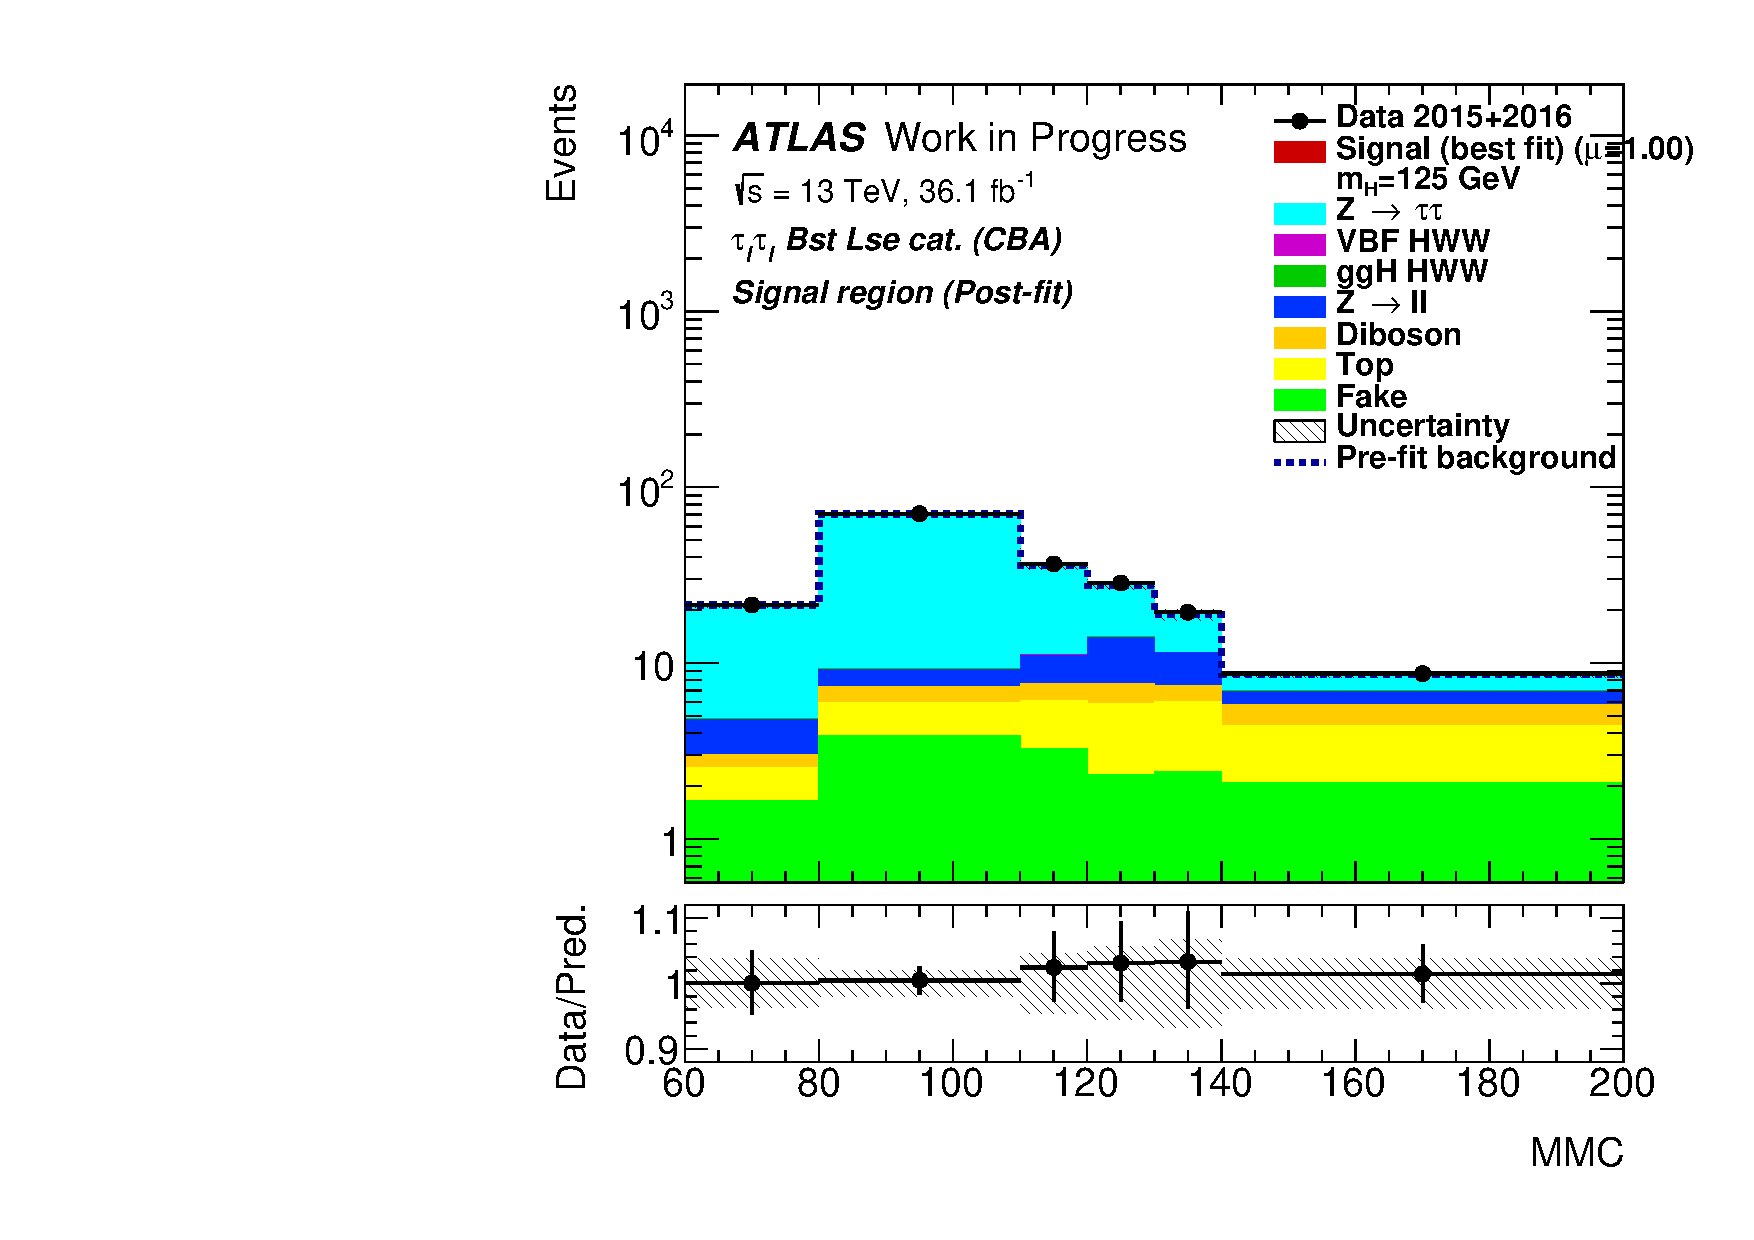
\includegraphics[width=\textwidth]{./plots/fit/cba/sig_boostloose.pdf}
        \caption{low boosted}
    \end{subfigure}
    \begin{subfigure}[t]{0.45\textwidth}
        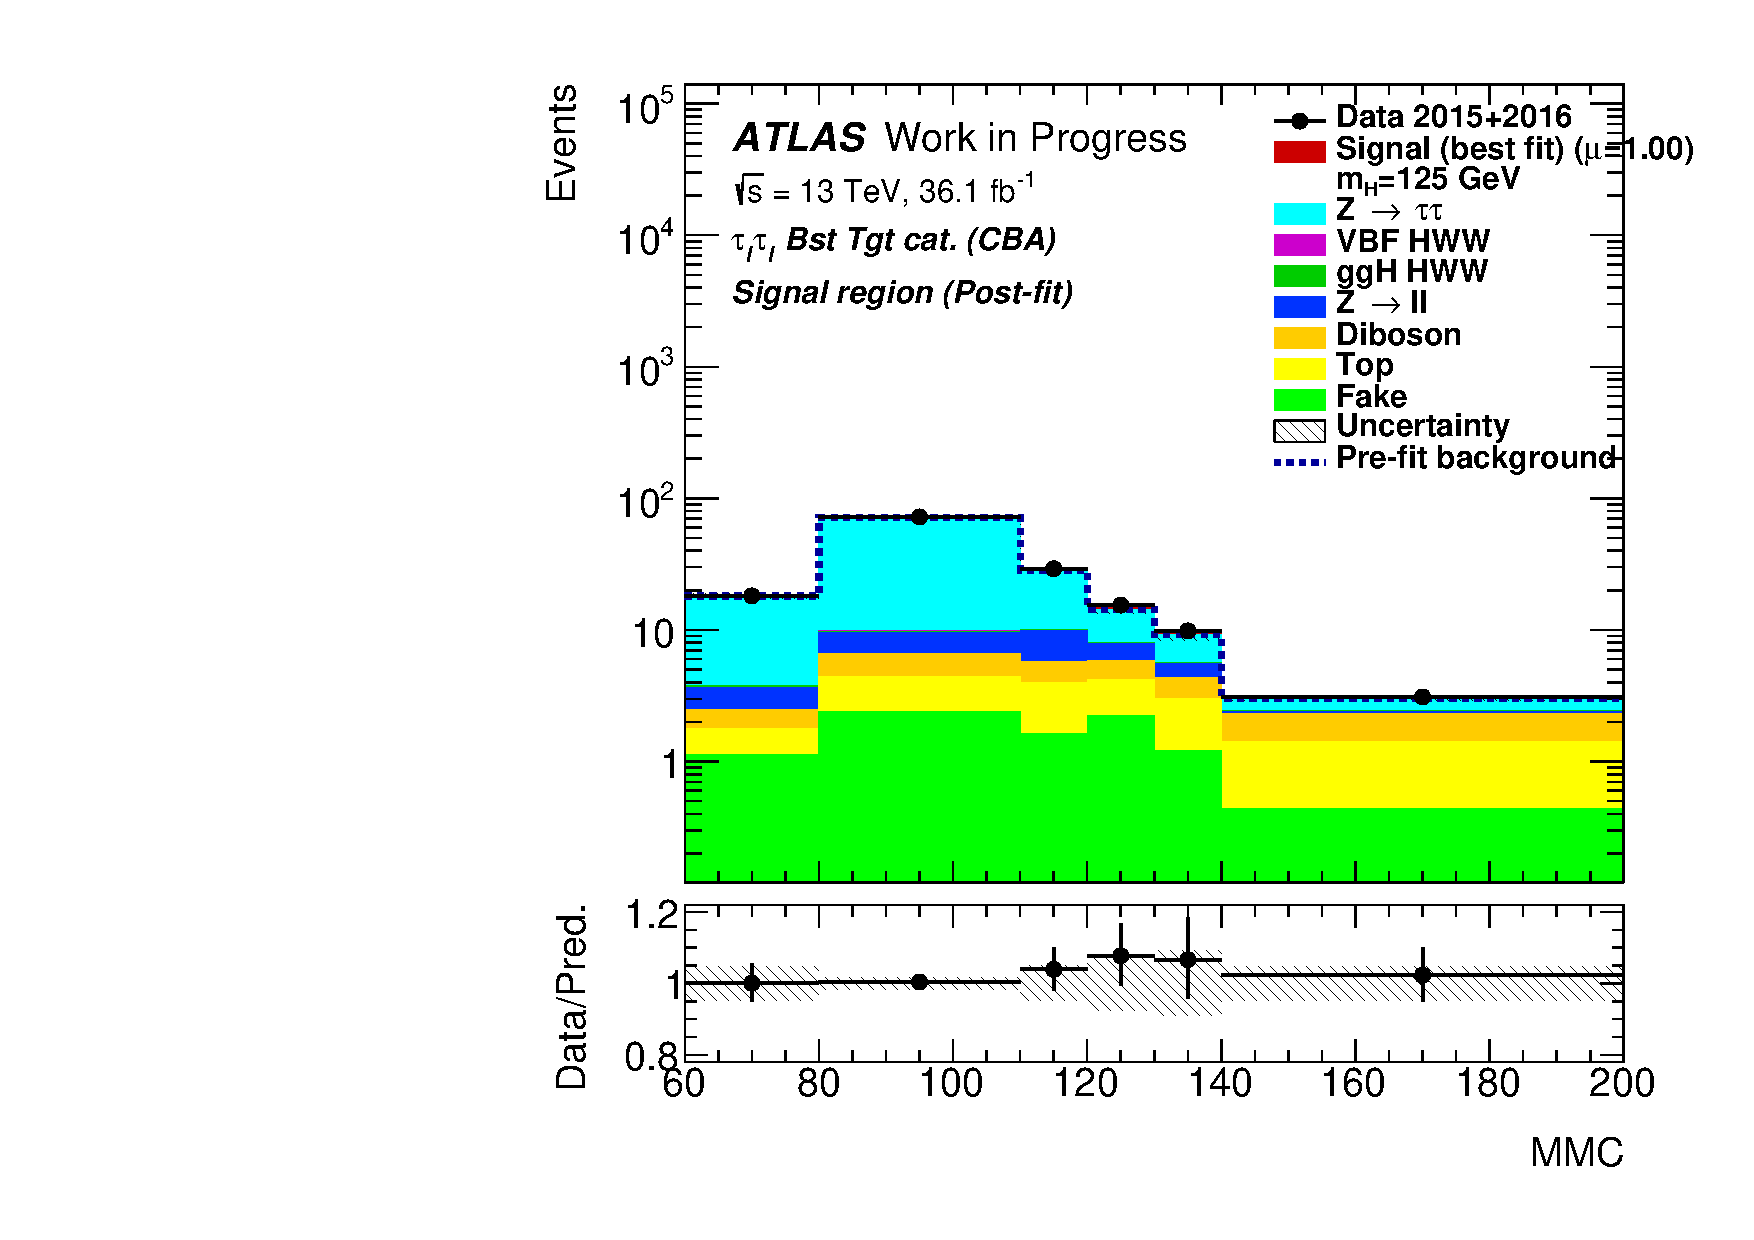
\includegraphics[width=\textwidth]{./plots/fit/cba/sig_boosttight.pdf}
        \caption{high boosted}
    \end{subfigure}
    \begin{subfigure}[t]{0.45\textwidth}
        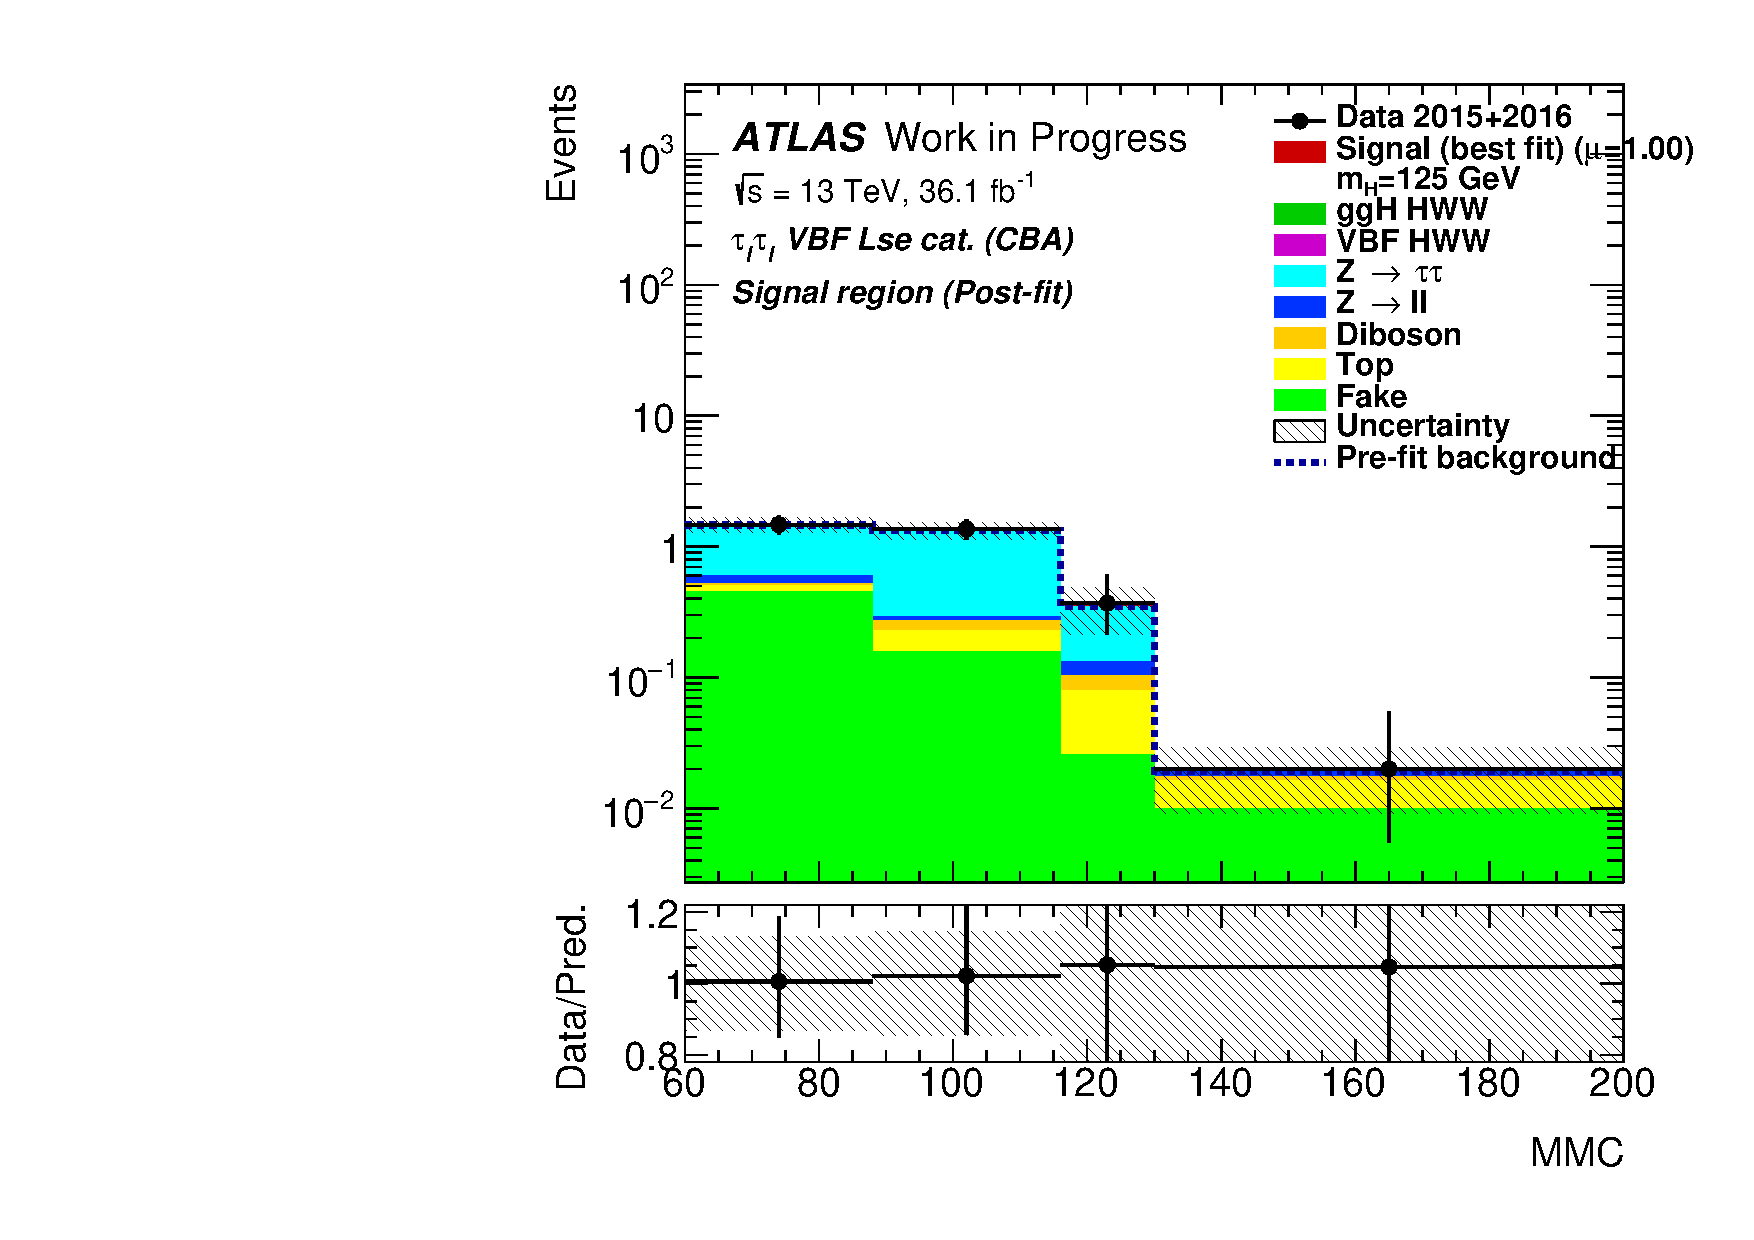
\includegraphics[width=\textwidth]{./plots/fit/cba/sig_vbfloose.pdf}
        \caption{low VBF}
    \end{subfigure}
    \begin{subfigure}[t]{0.45\textwidth}
        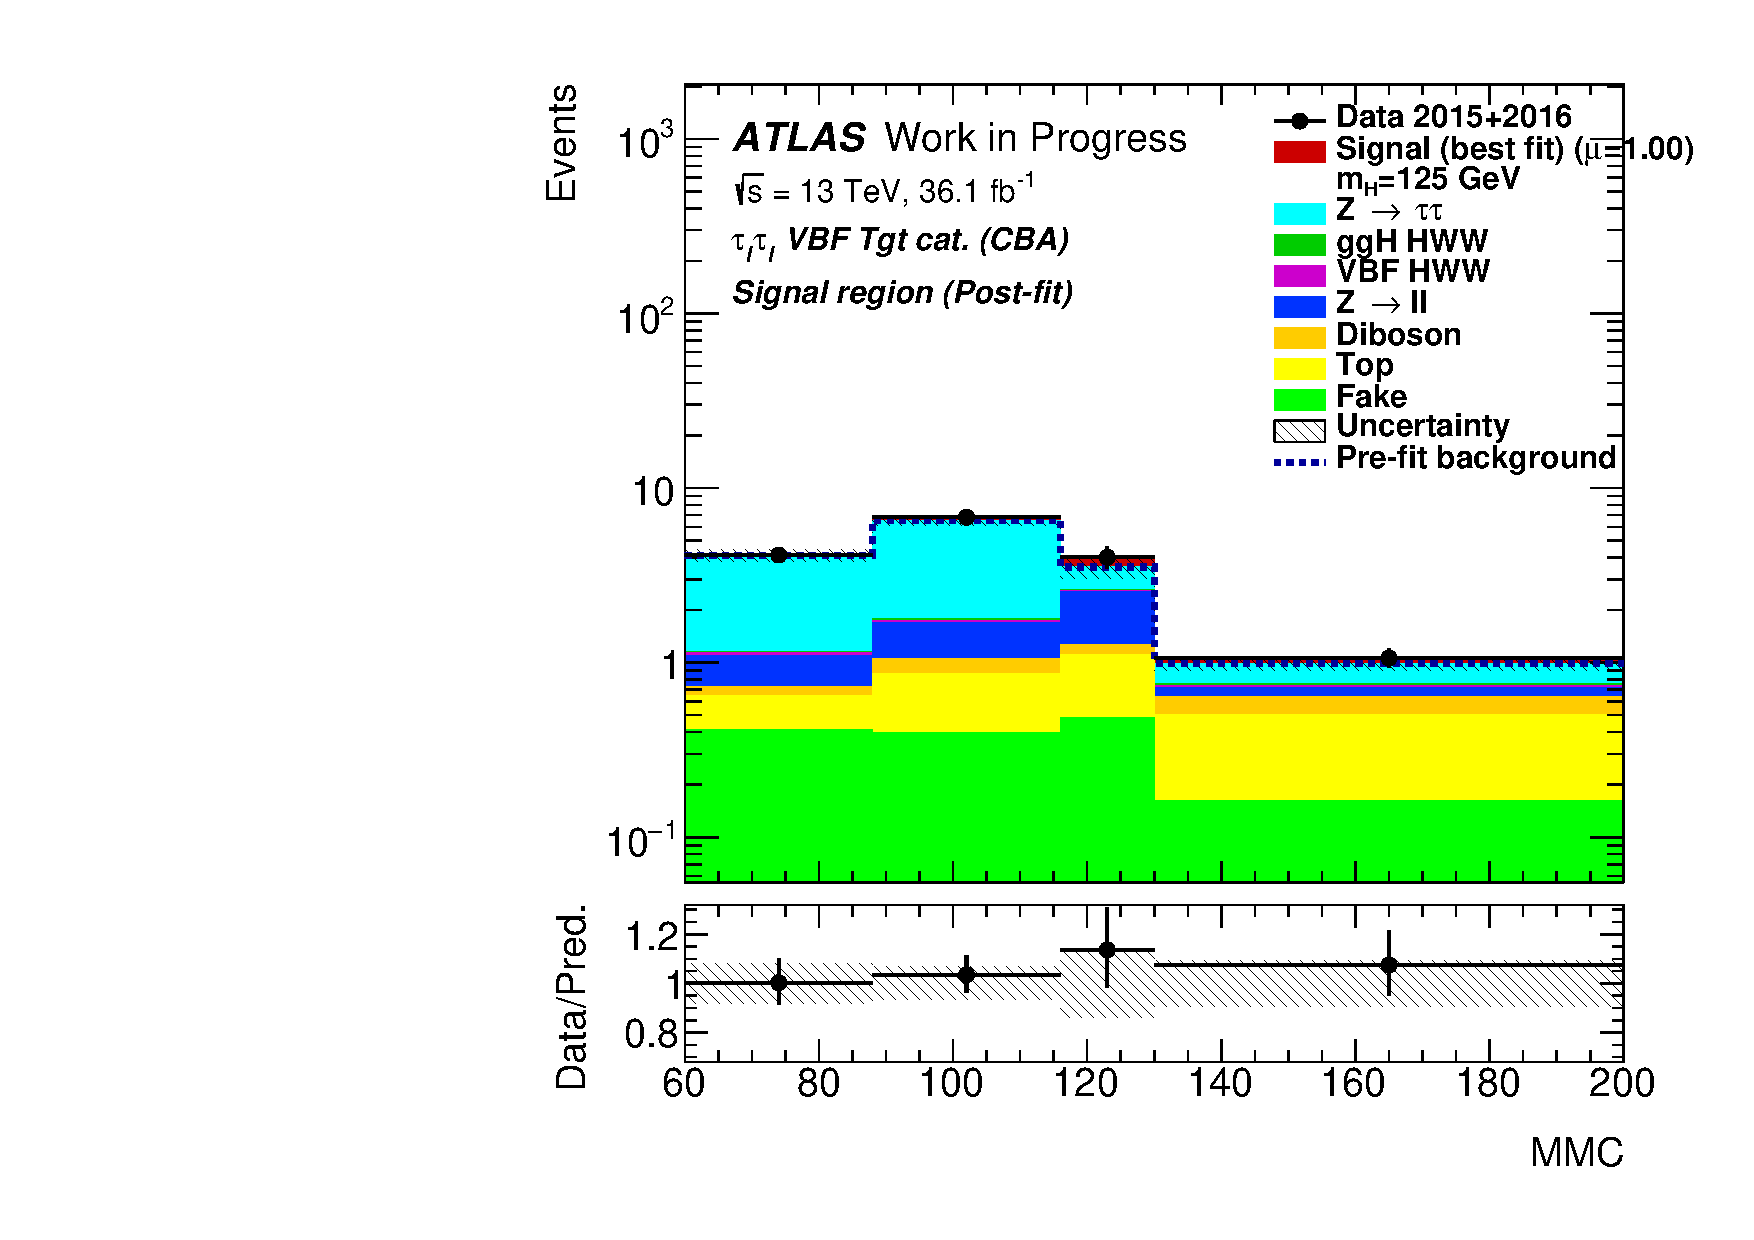
\includegraphics[width=\textwidth]{./plots/fit/cba/sig_vbftight.pdf}
        \caption{high VBF}
    \end{subfigure}
    \caption{Distributions of $\mmc$ in the different signal regions with the binning used in the fit of the cut-based analysis.
             For the data shown in the plot Asimov data corresponding to the 2015 and 2016 dataset with $\SI{36.1}{\invfb}$ are used.}\label{fig:fit:input:cba:SR}
\end{figure}

\begin{figure}[htb]
    \centering
    \begin{subfigure}[t]{0.45\textwidth}
        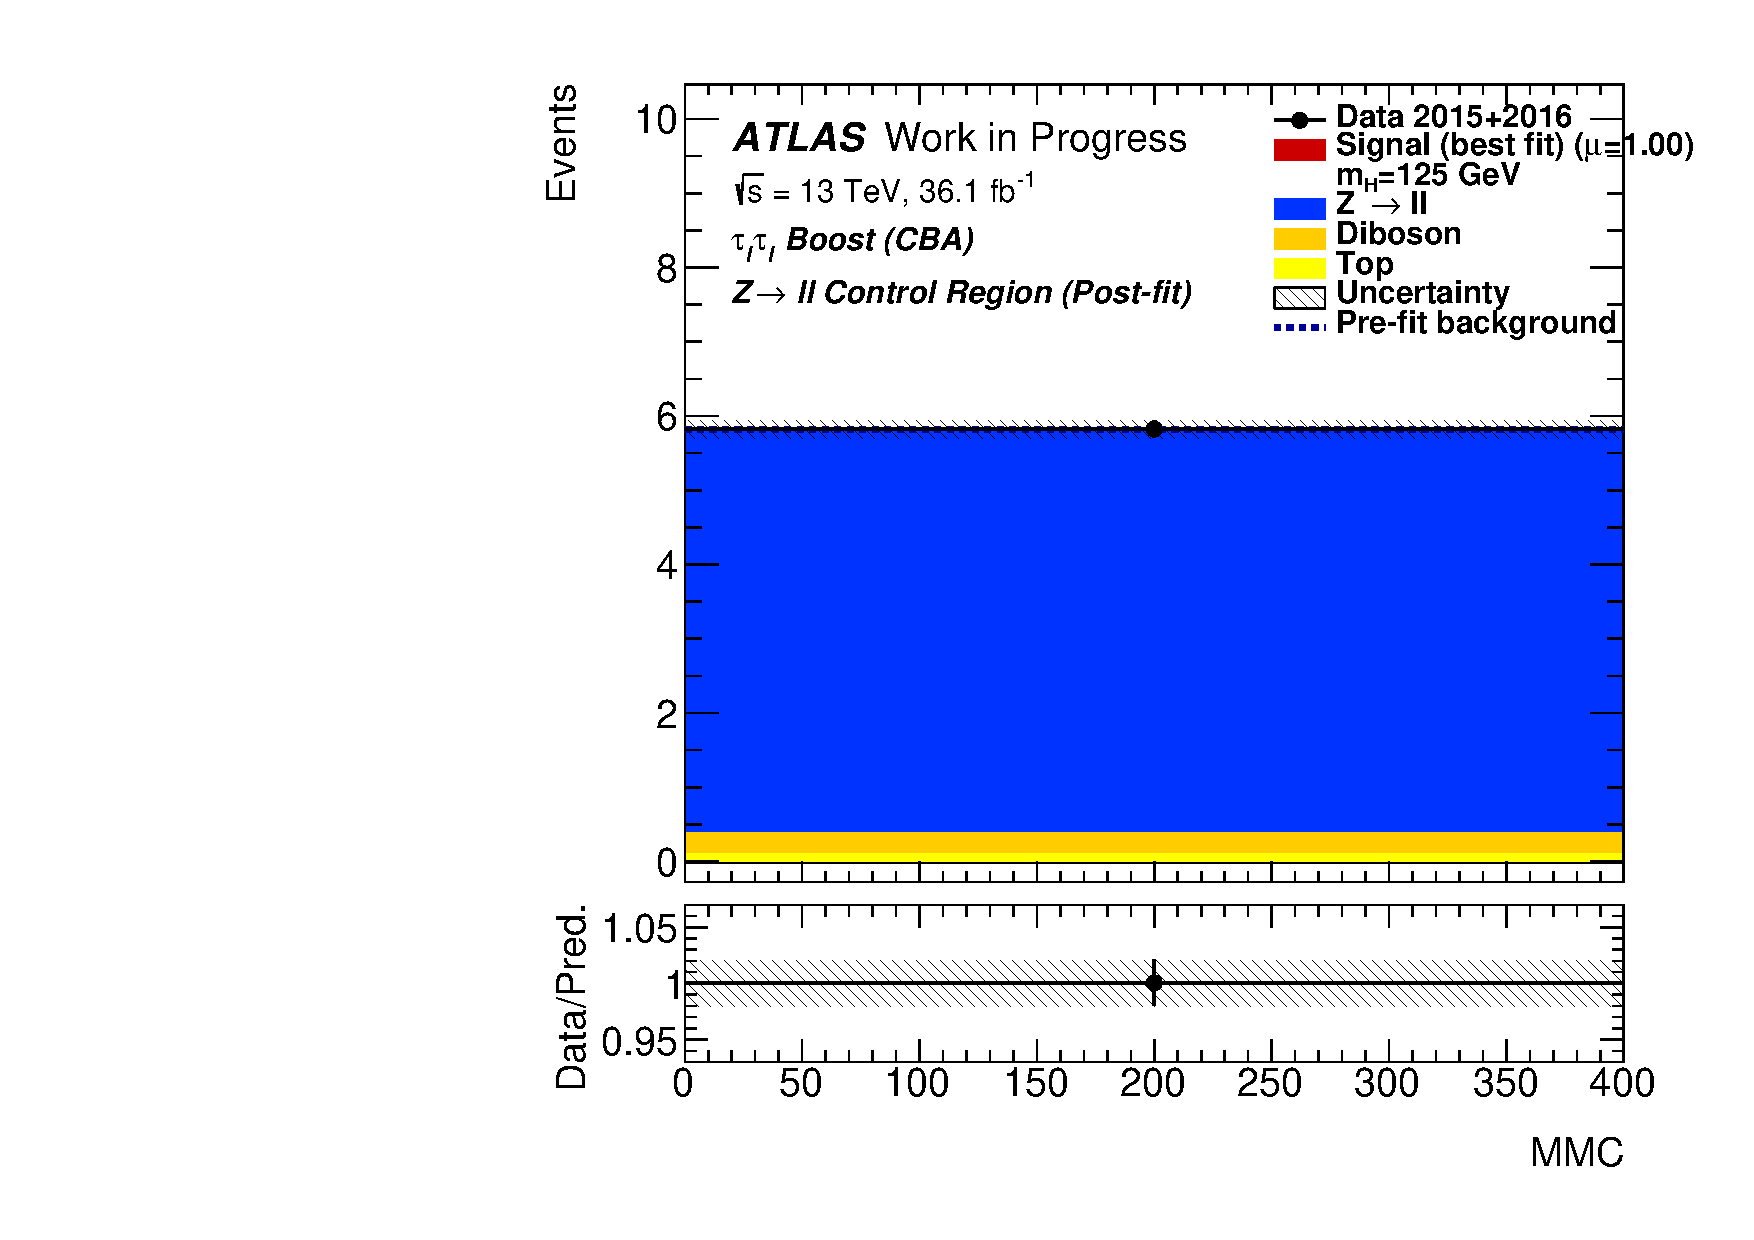
\includegraphics[width=\textwidth]{./plots/fit/cba/zll_boost.pdf}
        \caption{$\Zll$ boosted}
    \end{subfigure}
    \begin{subfigure}[t]{0.45\textwidth}
        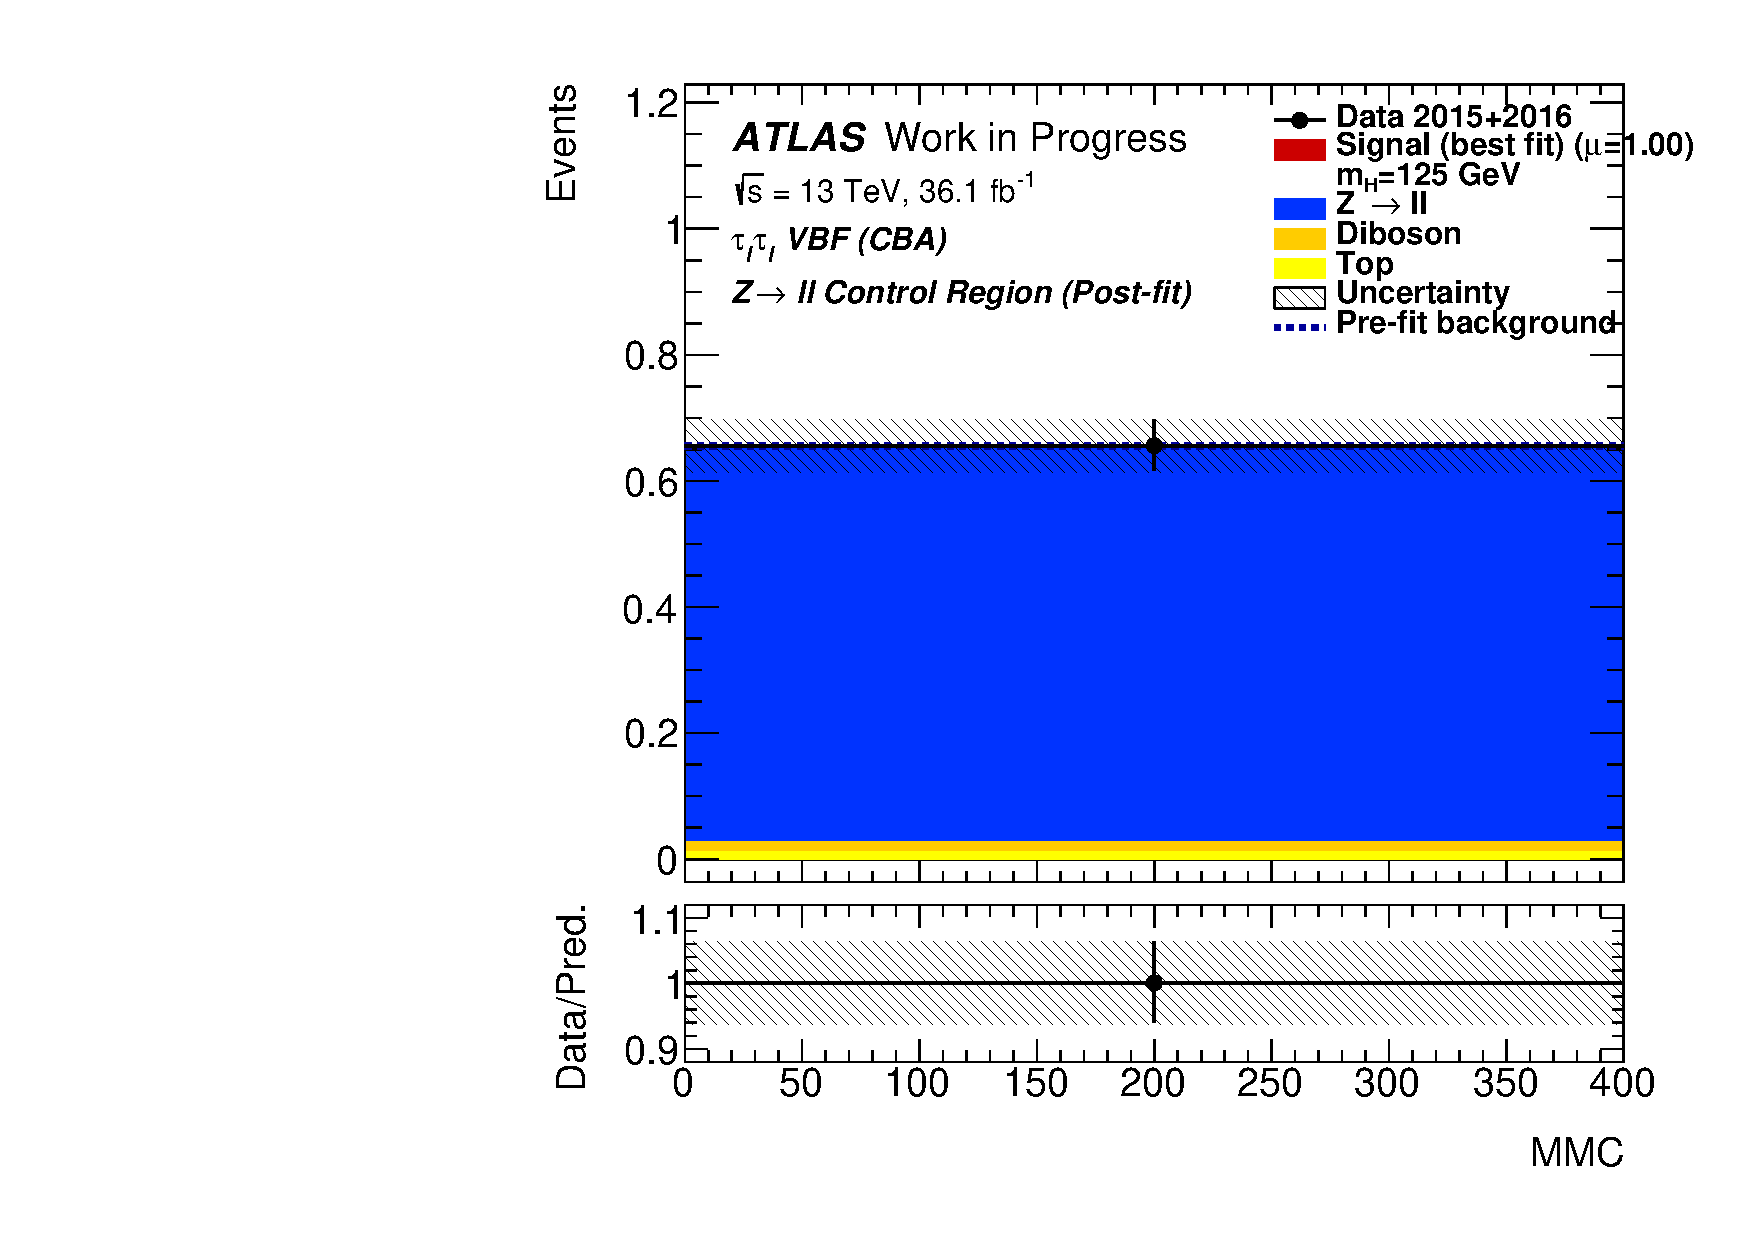
\includegraphics[width=\textwidth]{./plots/fit/cba/zll_vbf.pdf}
        \caption{$\Zll$ VBF}
    \end{subfigure}
    \begin{subfigure}[t]{0.45\textwidth}
        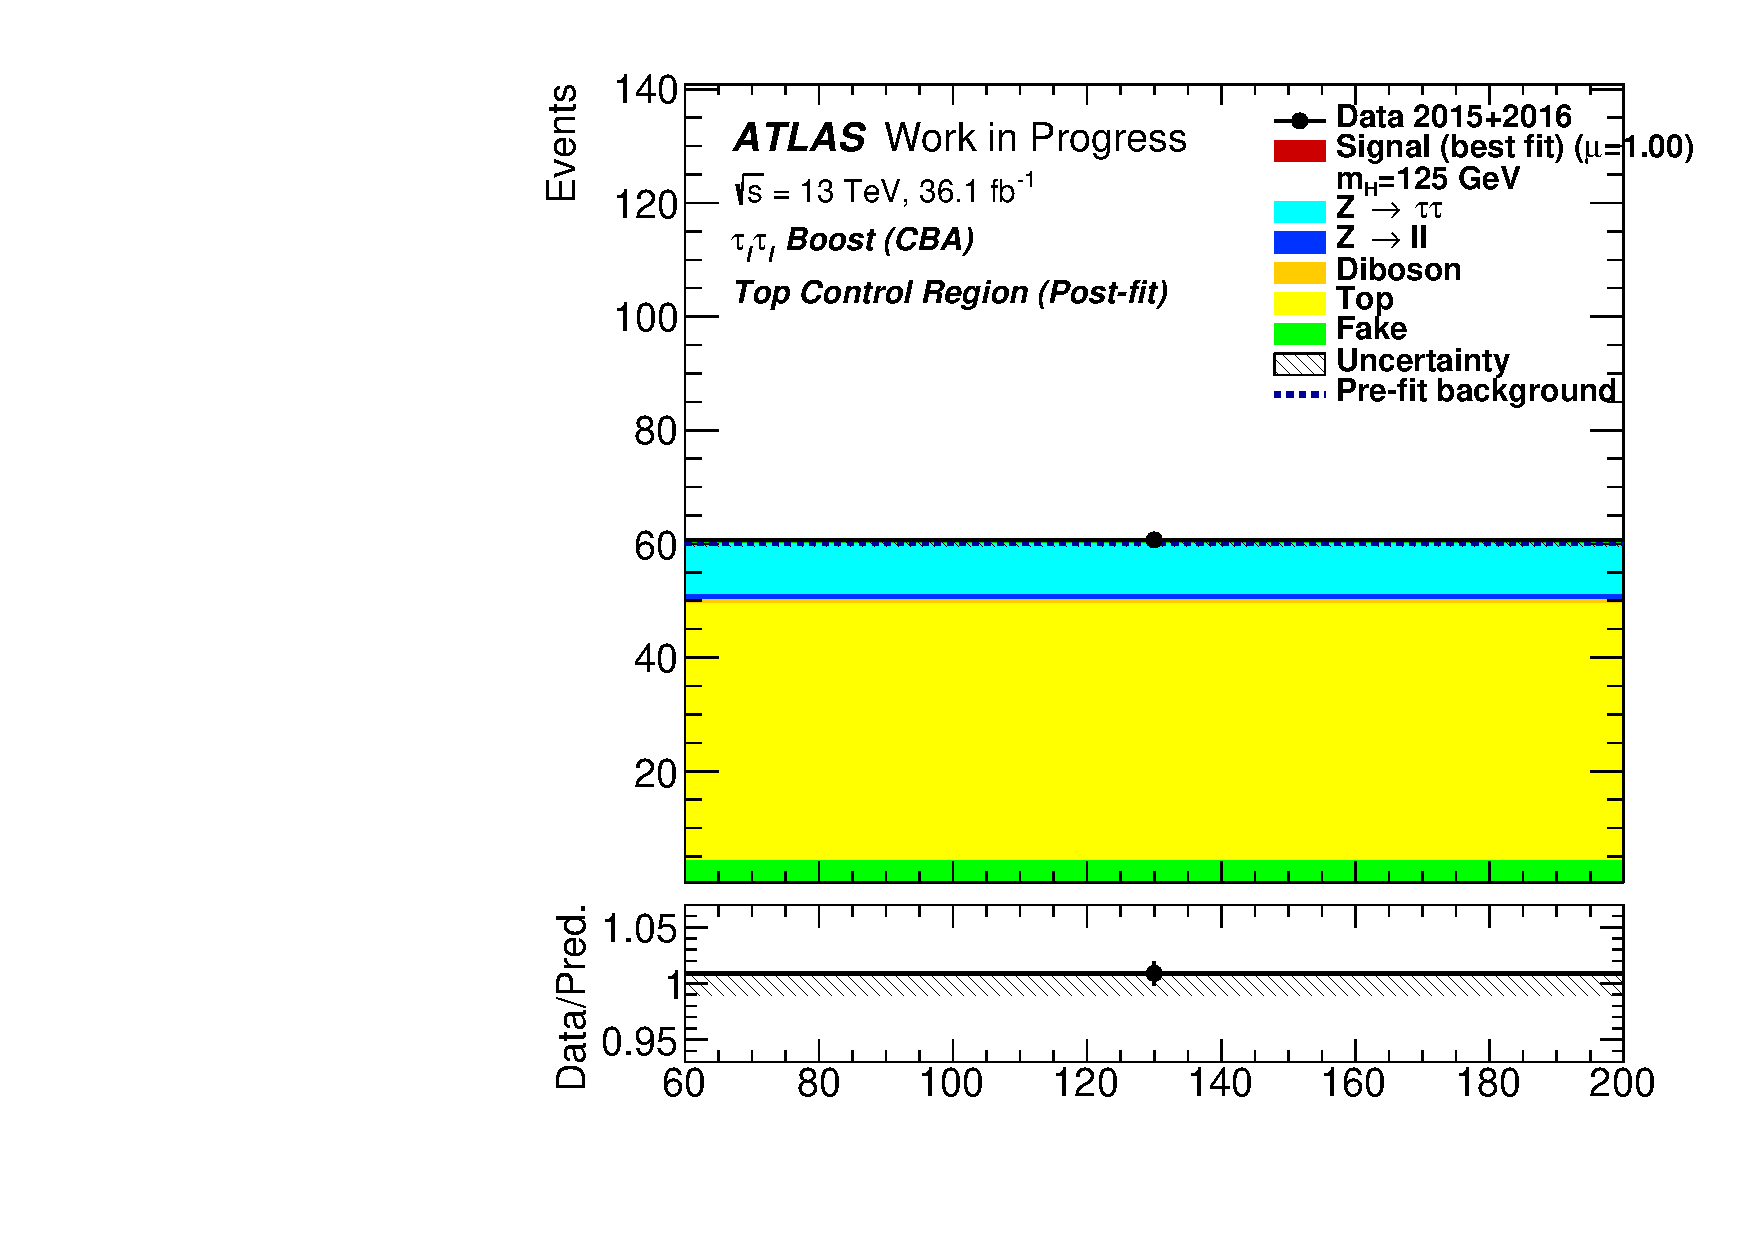
\includegraphics[width=\textwidth]{./plots/fit/cba/top_boost.pdf}
        \caption{Top boosted}
    \end{subfigure}
    \begin{subfigure}[t]{0.45\textwidth}
        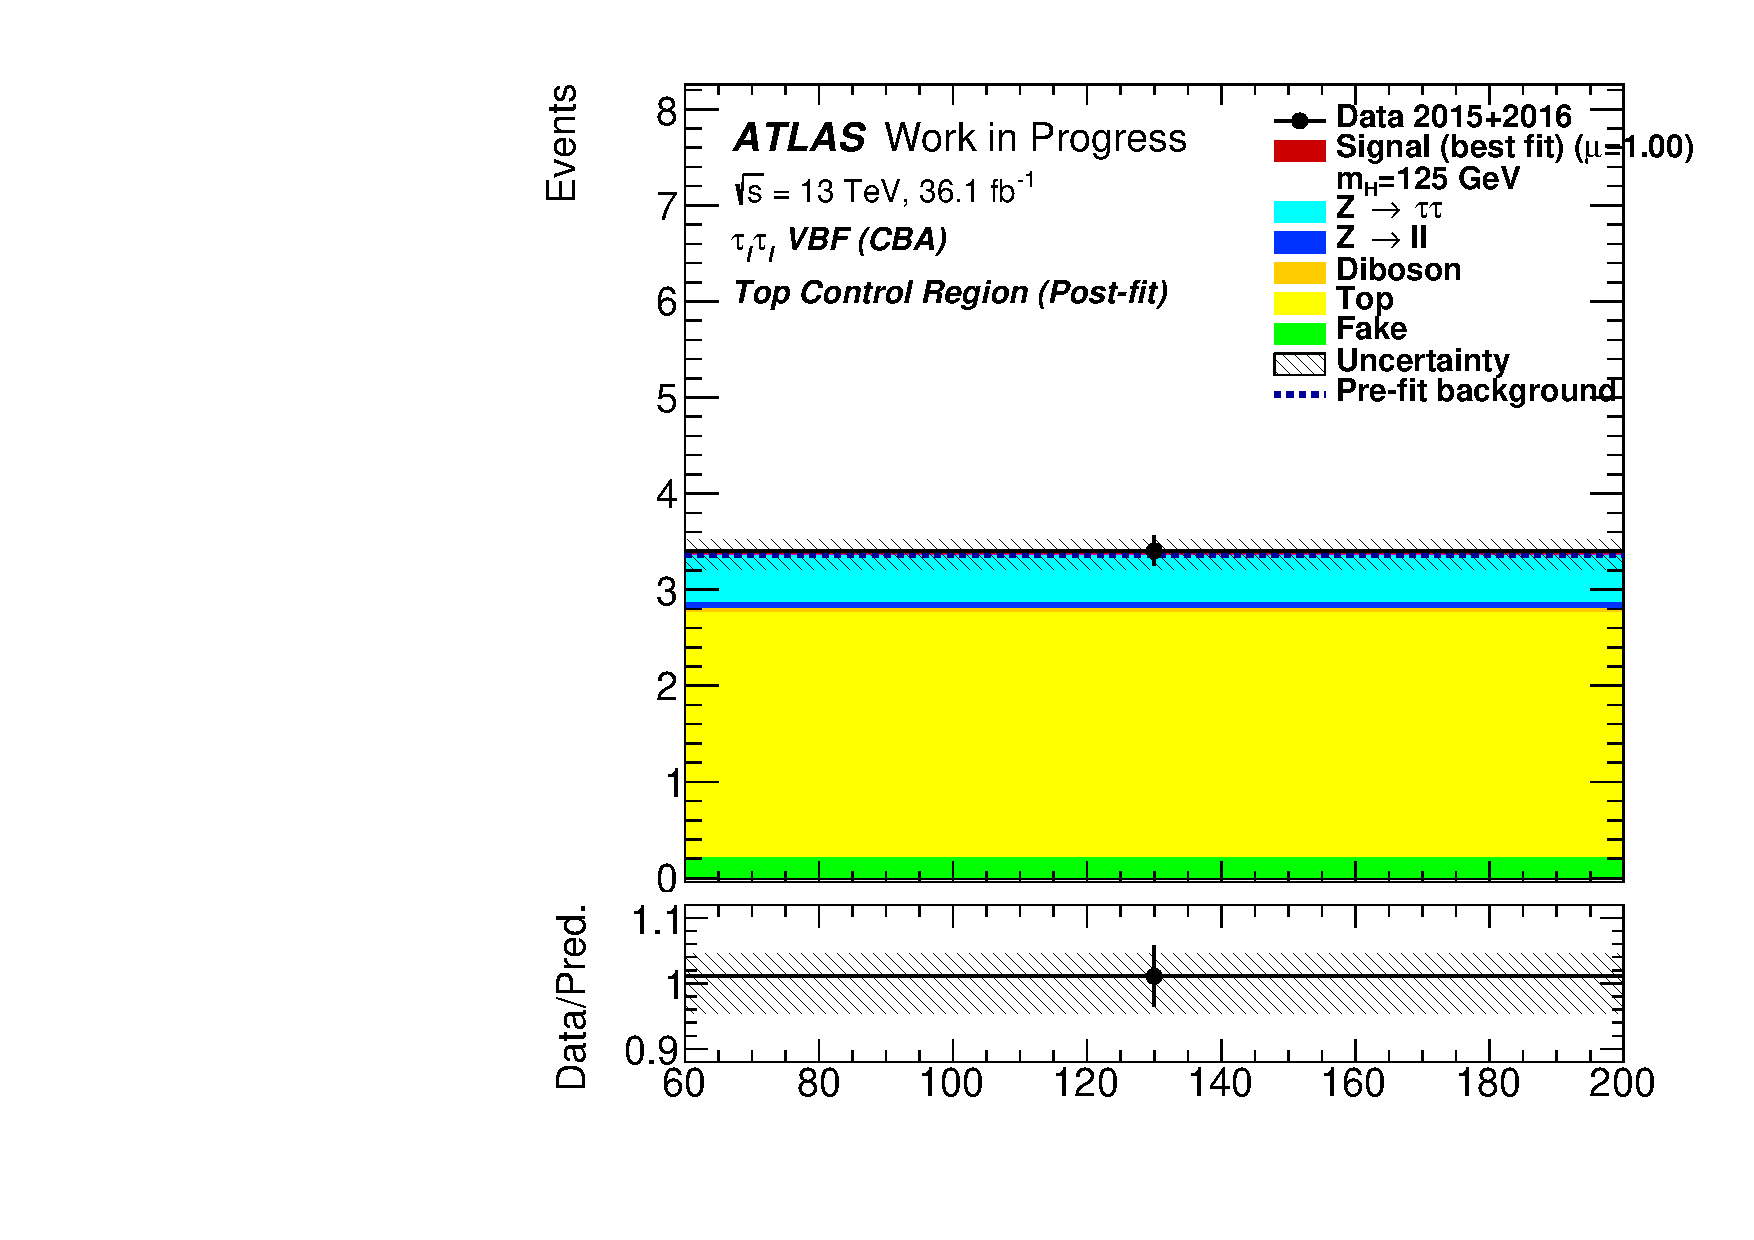
\includegraphics[width=\textwidth]{./plots/fit/cba/top_vbf.pdf}
        \caption{Top VBF}
    \end{subfigure}

    \caption{Distributions of $\mmc$ in the different control regions with the binning used in the fit of the cut-based analysis.
             For the data shown in the plot Asimov data corresponding to the 2015 and 2016 dataset with $\SI{36.1}{\invfb}$ are used.}\label{fig:fit:input:cba:CR}
\end{figure}


\begin{figure}[htb]
    \centering
    \begin{subfigure}[t]{0.45\textwidth}
        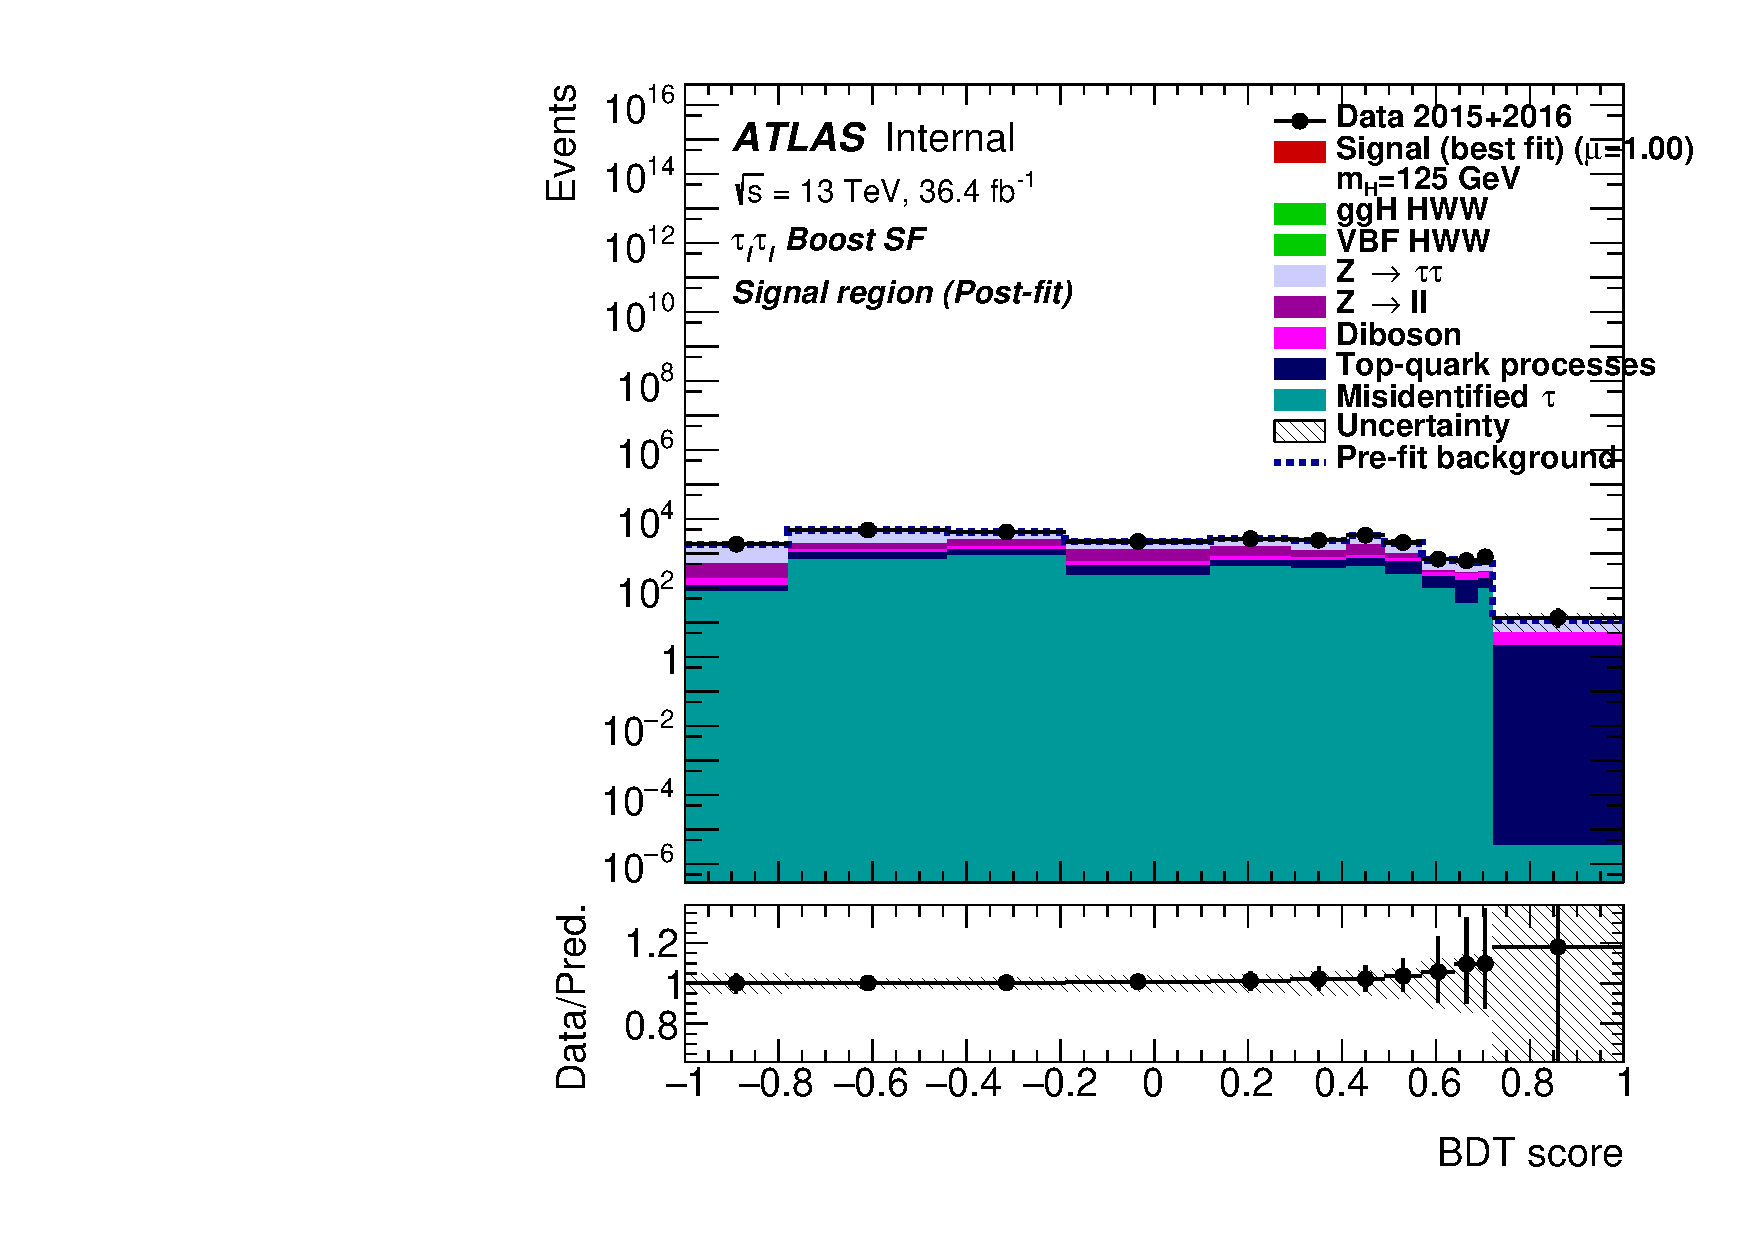
\includegraphics[width=\textwidth]{./plots/fit/mva/sig_boostsf.pdf}
        \caption{Boosted SF}
    \end{subfigure}
    \begin{subfigure}[t]{0.45\textwidth}
        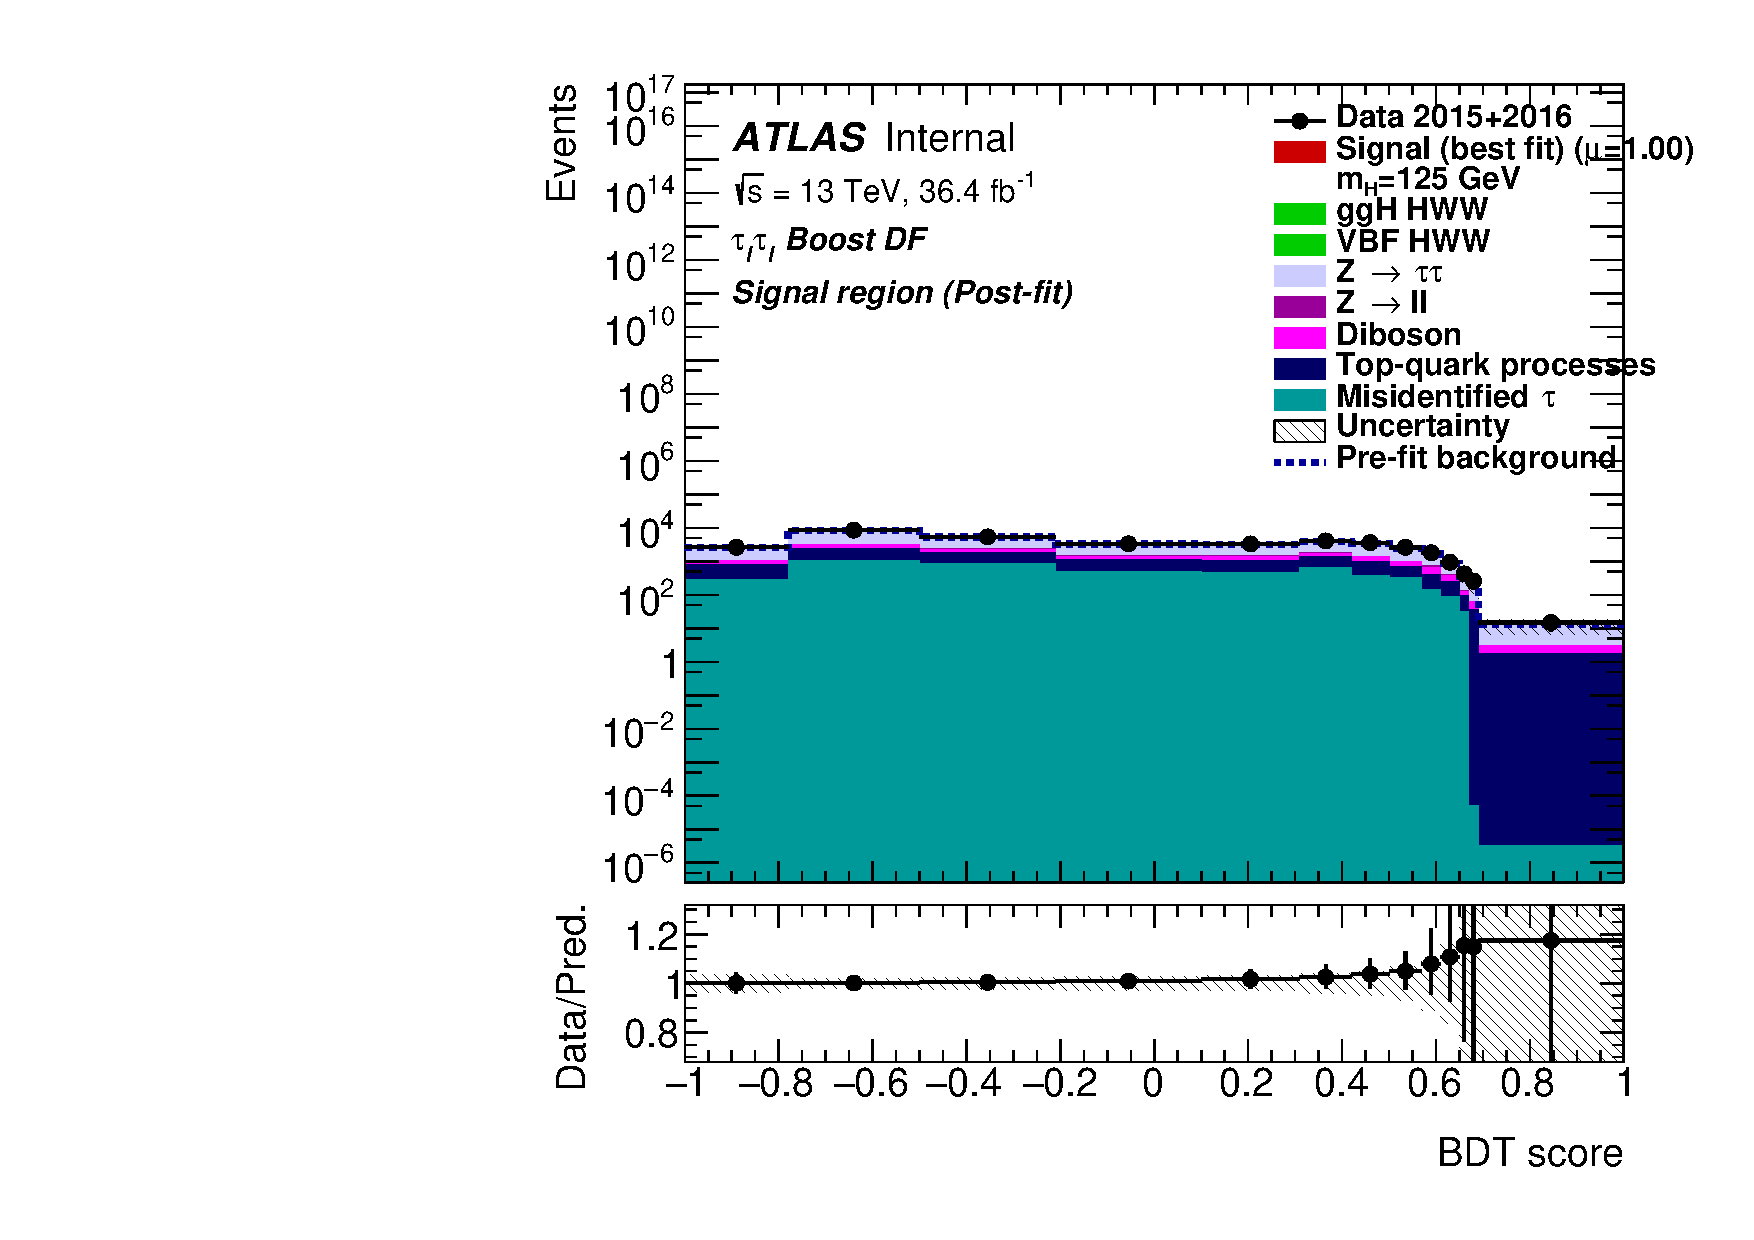
\includegraphics[width=\textwidth]{./plots/fit/mva/sig_boostdf.pdf}
        \caption{Boosted DF}
    \end{subfigure}
    \begin{subfigure}[t]{0.45\textwidth}
        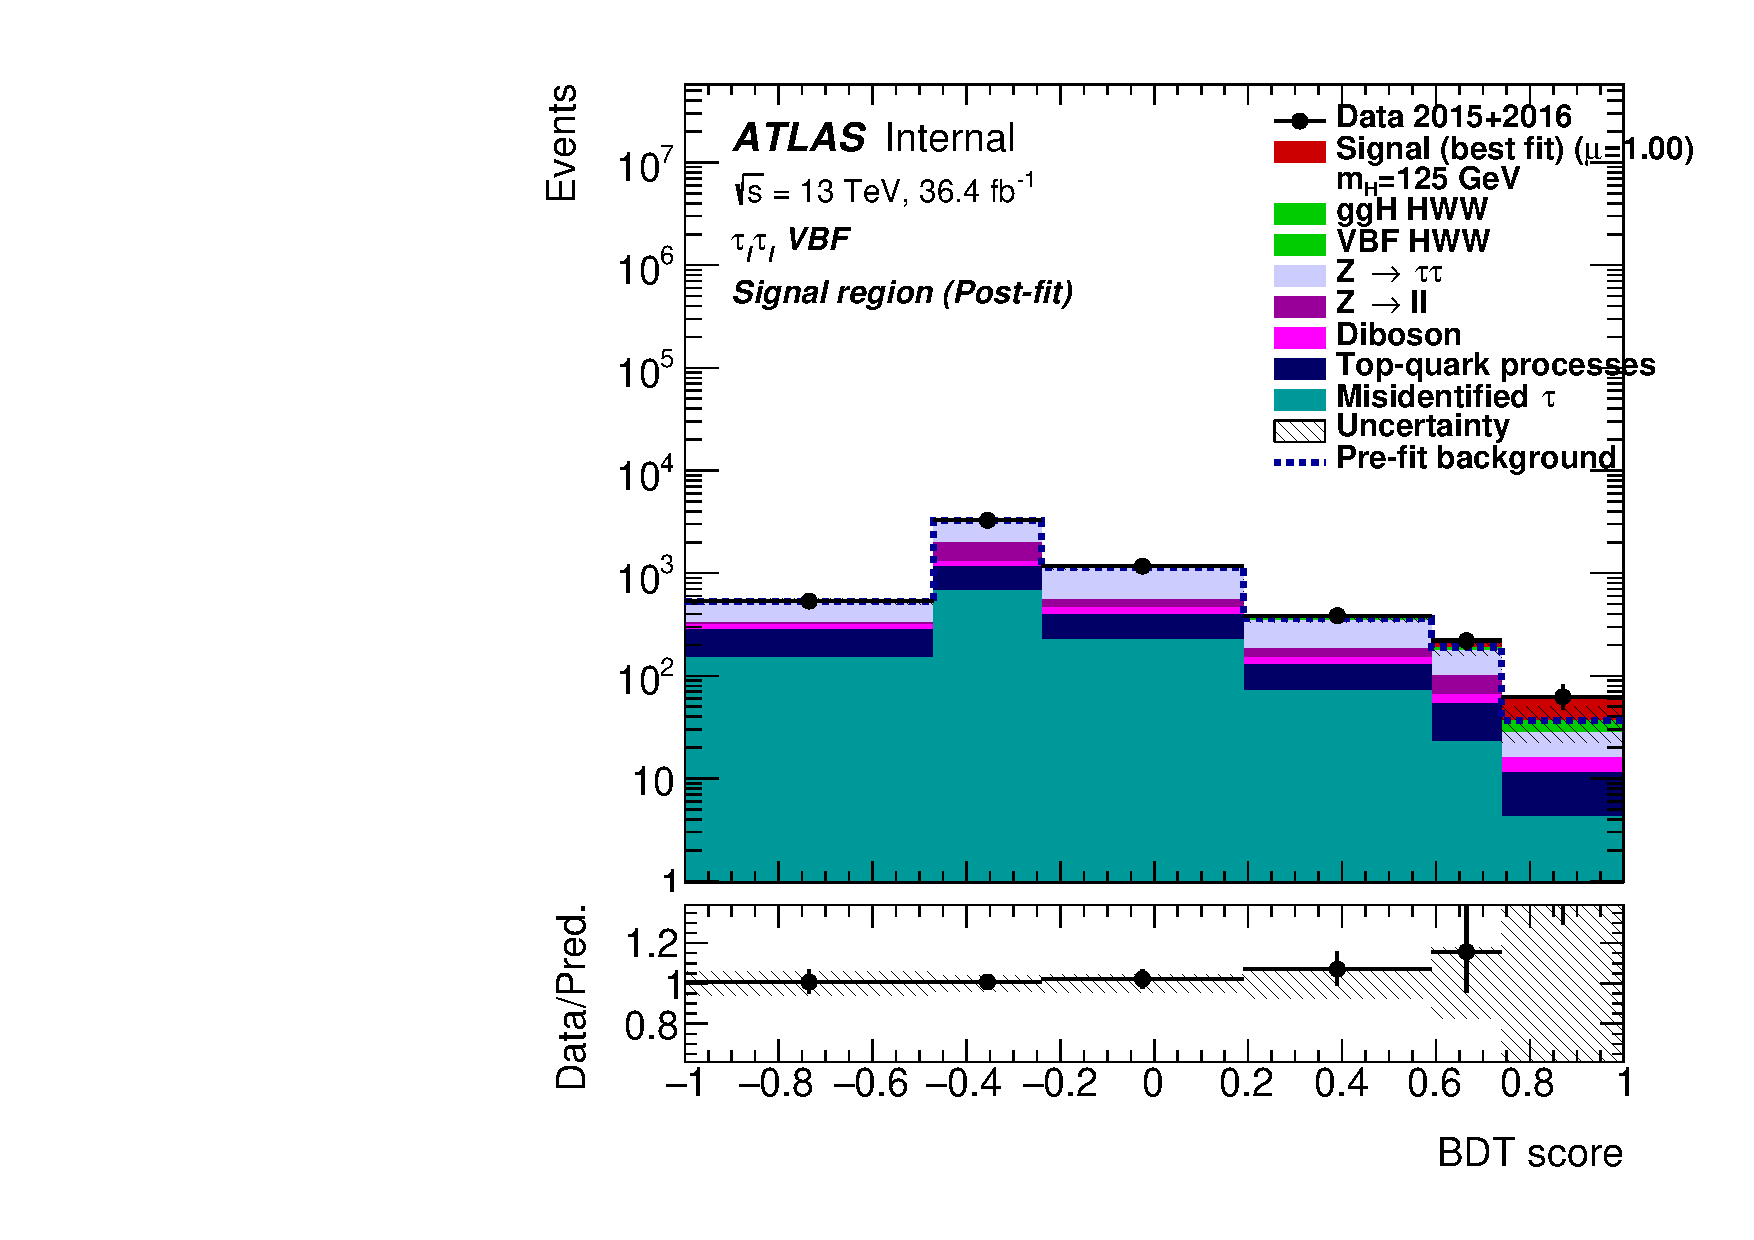
\includegraphics[width=\textwidth]{./plots/fit/mva/sig_vbf.pdf}
        \caption{VBF}
    \end{subfigure}
    \caption{Distributions of the BDT output in the different signal regions with the binning used in the fit of the multivariate analysis.
             For the data shown in the plot Asimov data corresponding to the 2015 and 2016 dataset with $\SI{36.1}{\invfb}$ are used.}\label{fig:fit:input:mva:SR}
\end{figure}

\begin{figure}[htb]
    \centering
    \begin{subfigure}[t]{0.45\textwidth}
        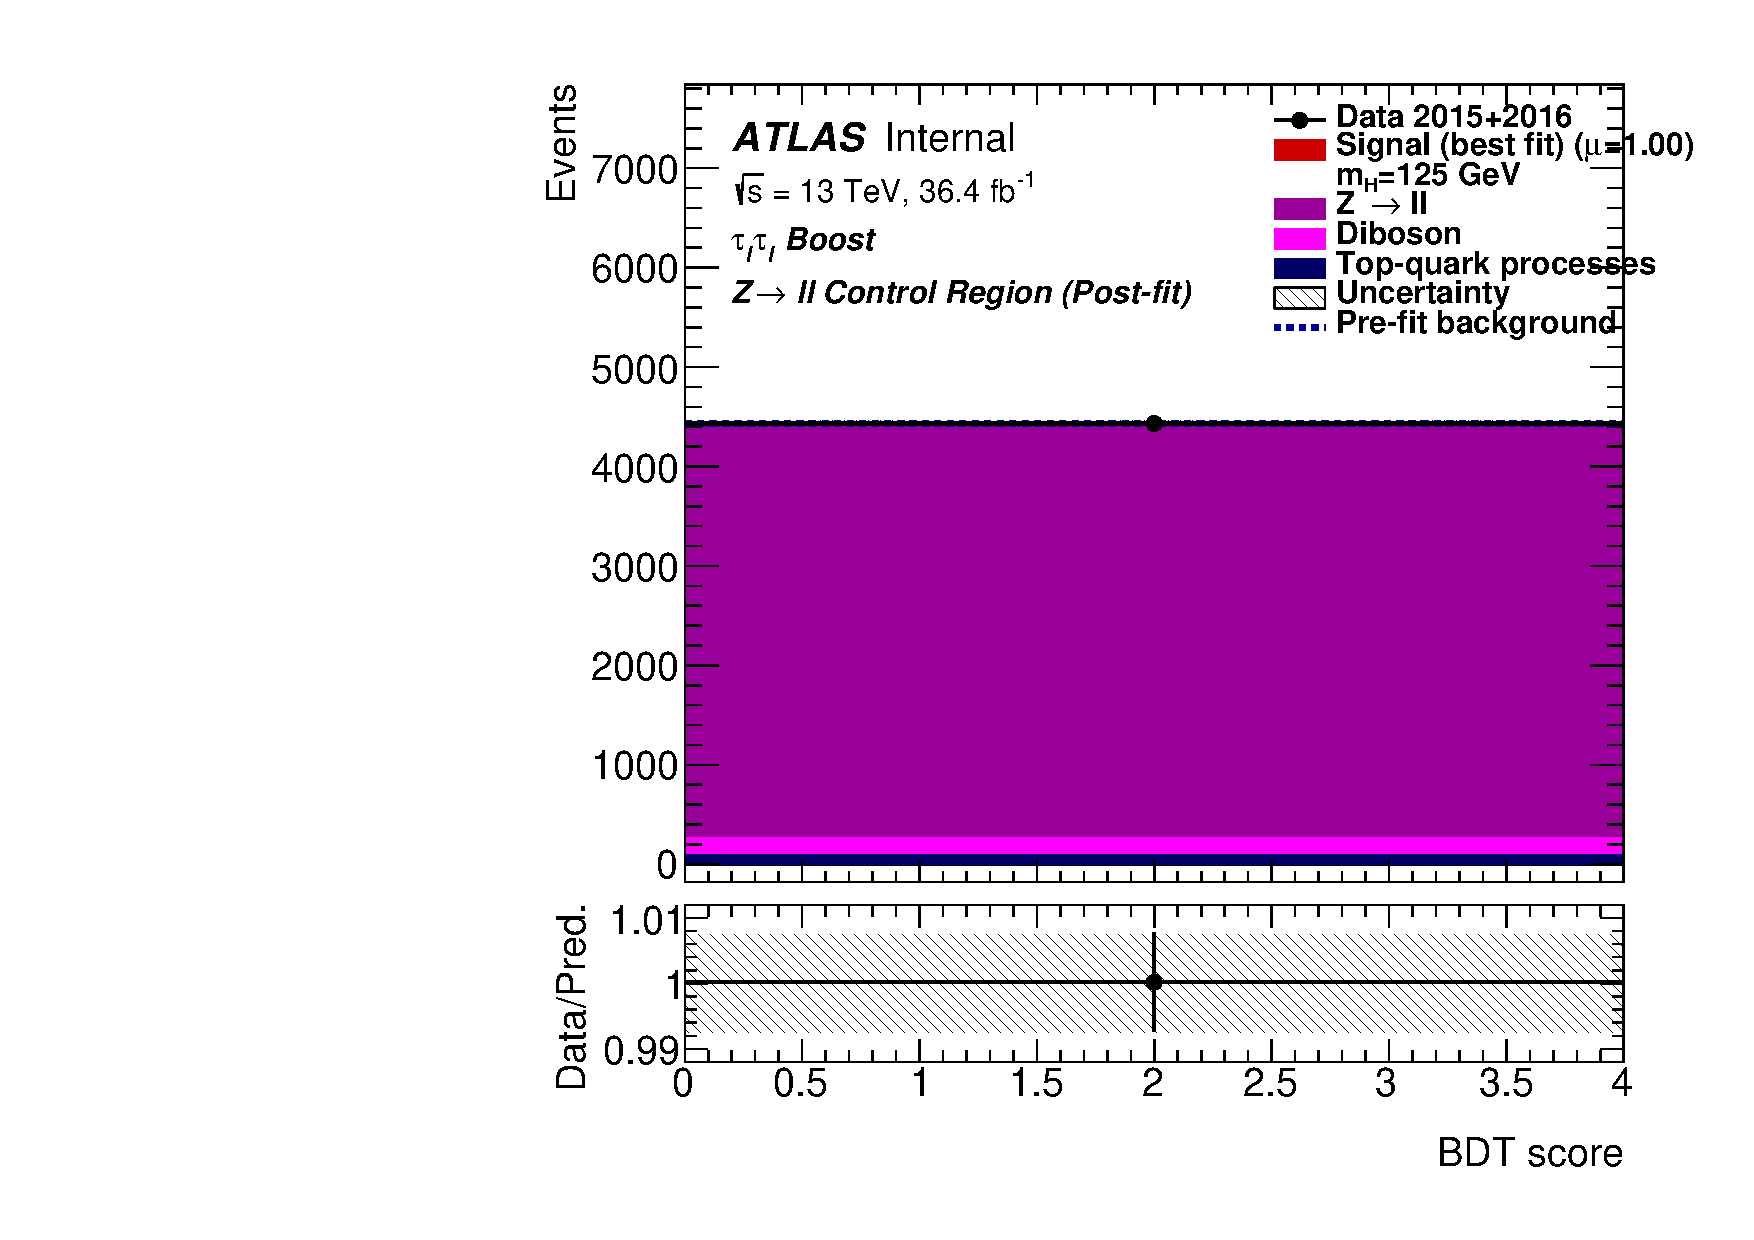
\includegraphics[width=\textwidth]{./plots/fit/mva/zll_boost.pdf}
        \caption{$\Zll$ boosted}
    \end{subfigure}
    \begin{subfigure}[t]{0.45\textwidth}
        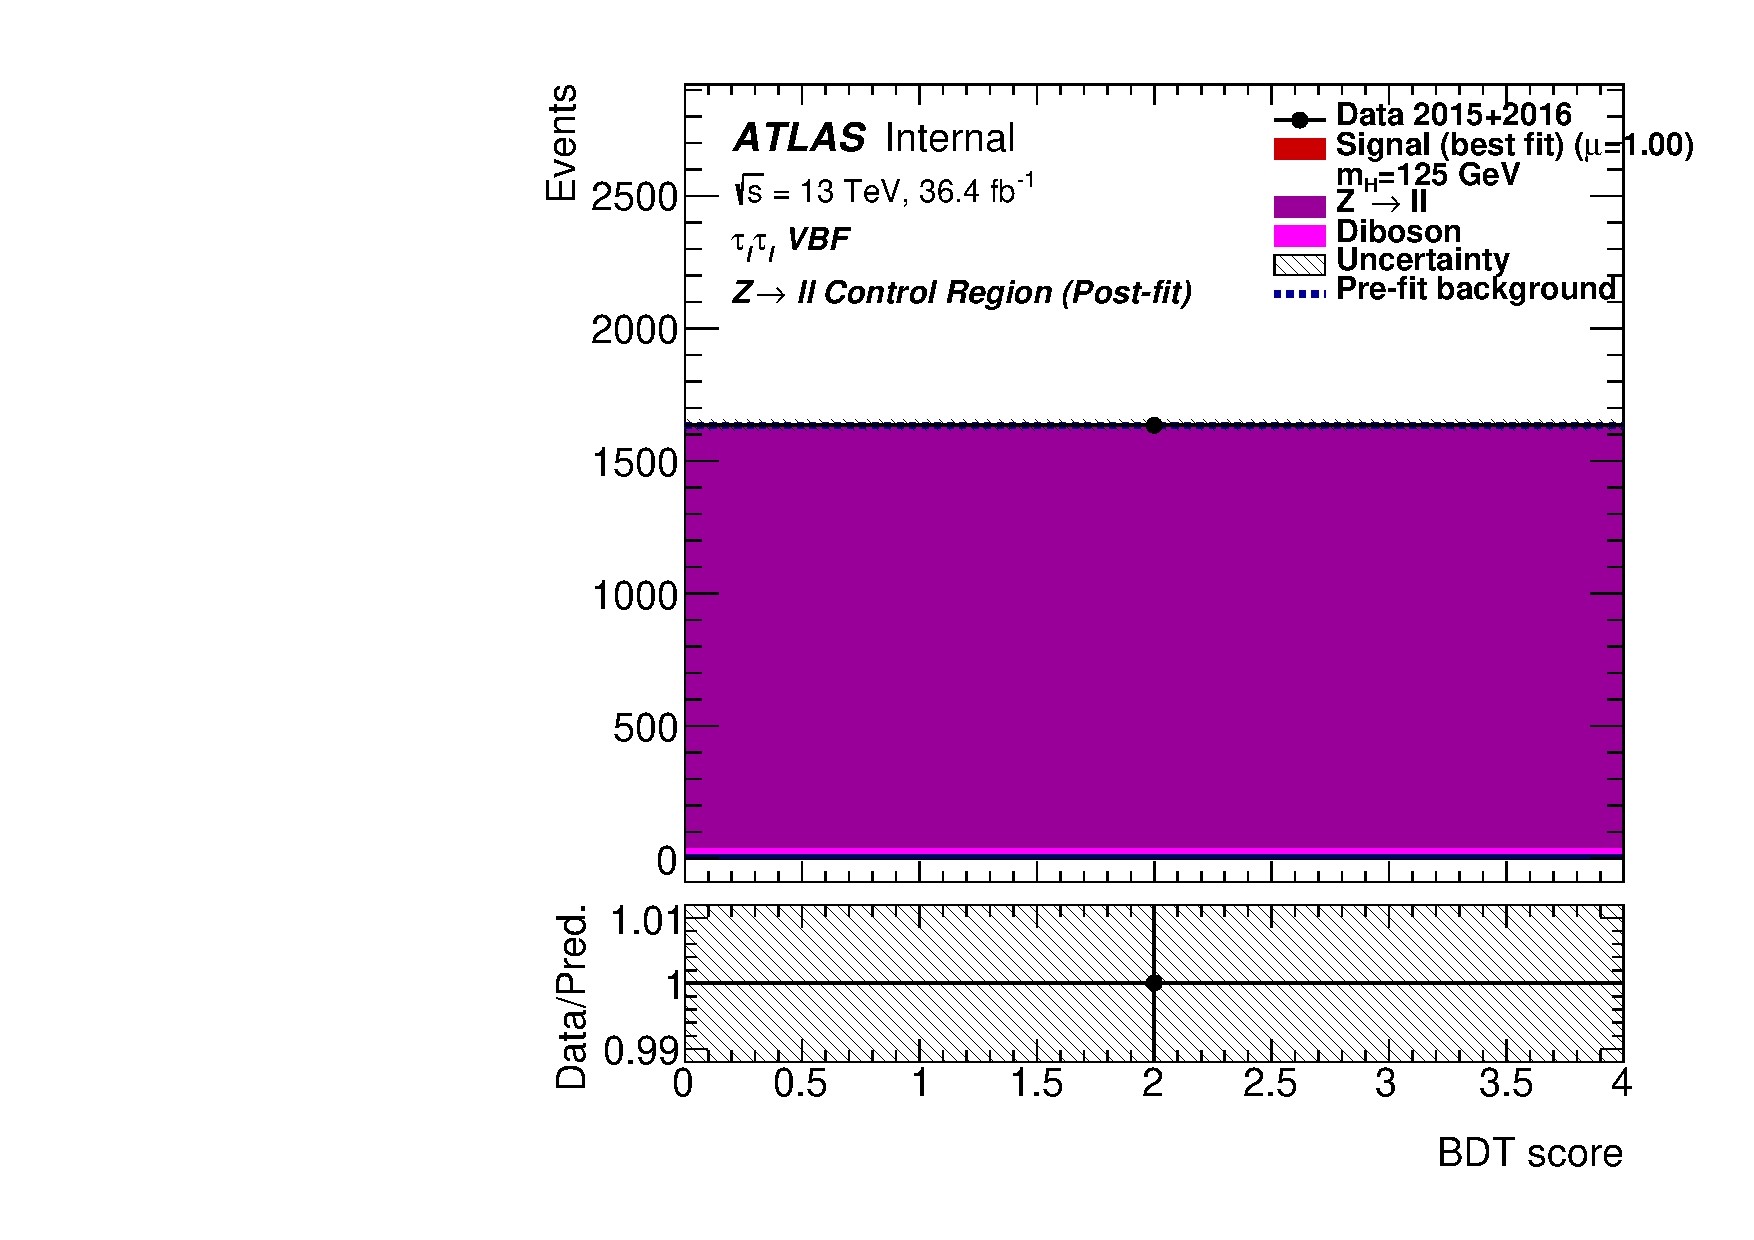
\includegraphics[width=\textwidth]{./plots/fit/mva/zll_vbf.pdf}
        \caption{$\Zll$ VBF}
    \end{subfigure}
    \begin{subfigure}[t]{0.45\textwidth}
        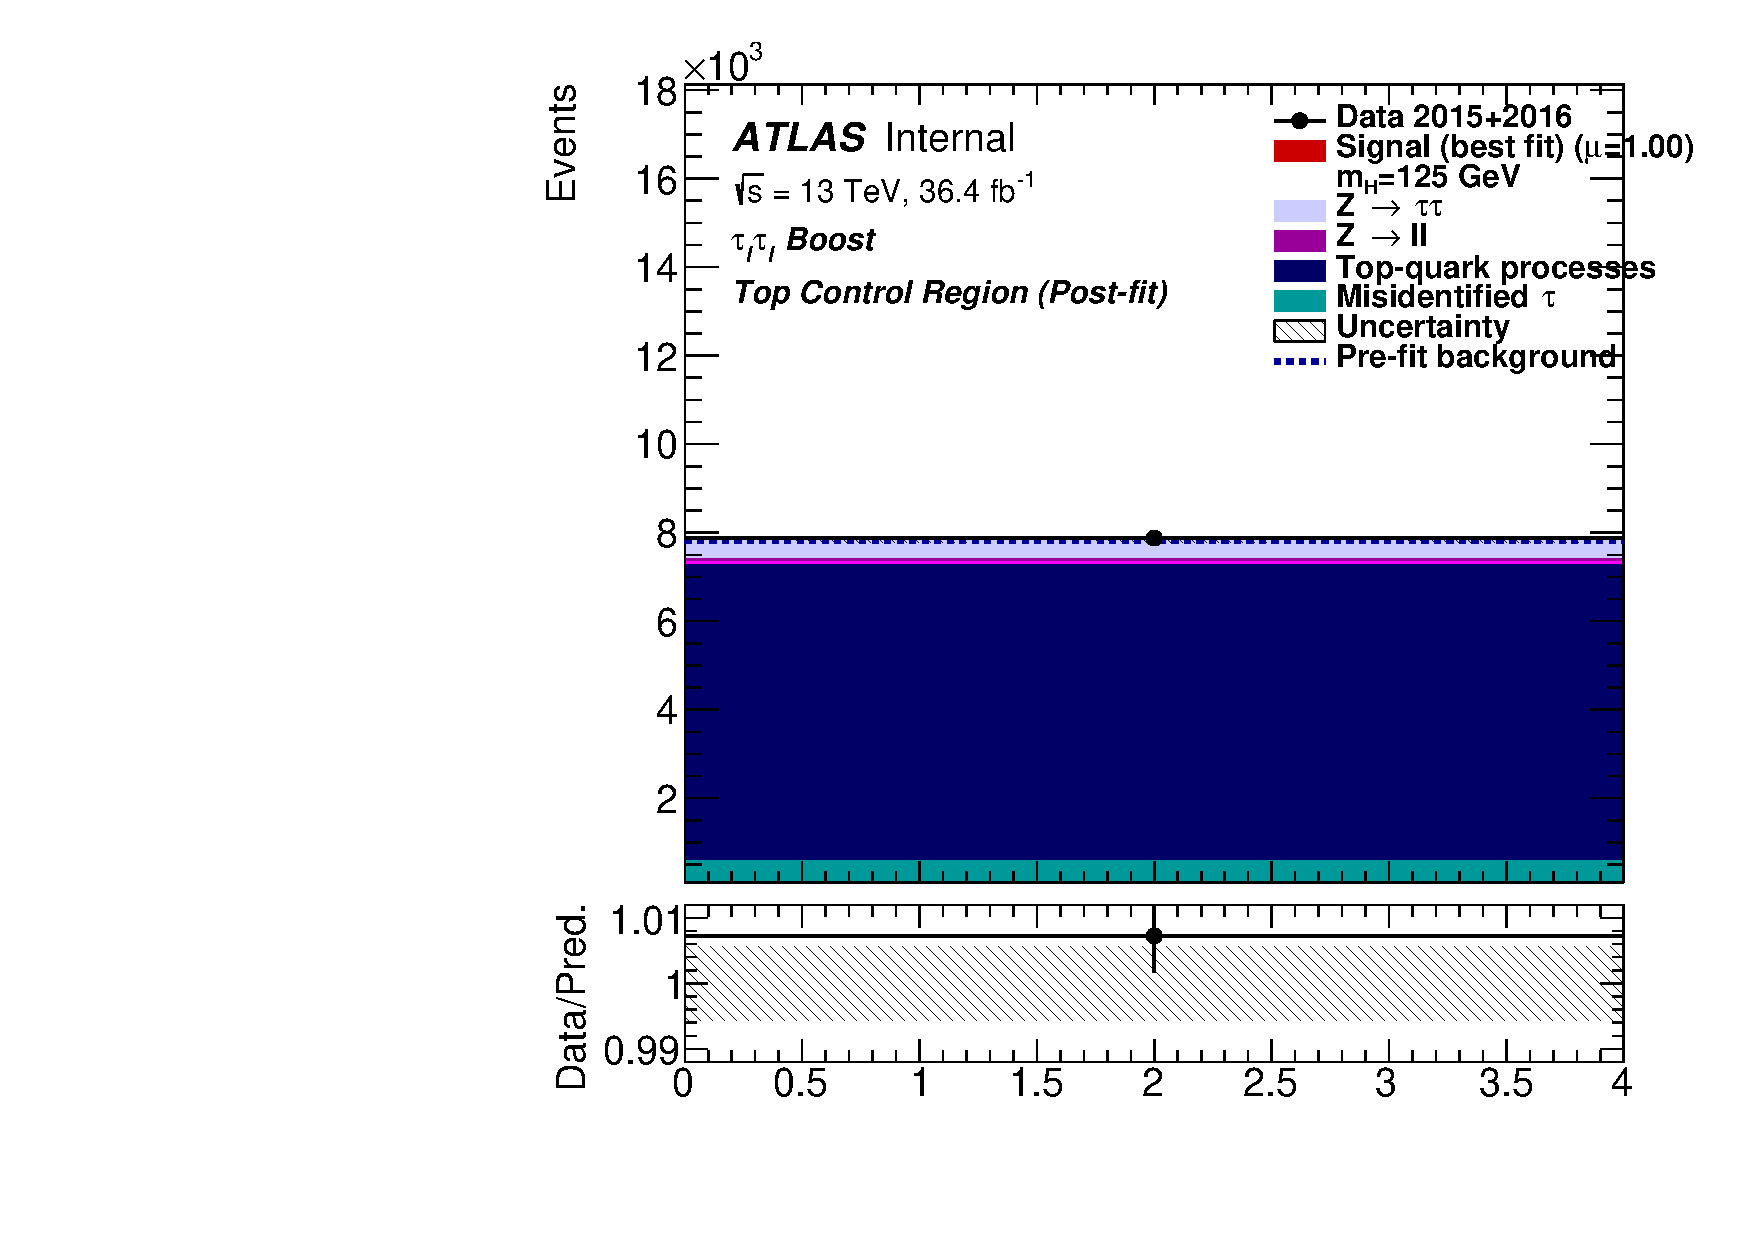
\includegraphics[width=\textwidth]{./plots/fit/mva/top_boost.pdf}
        \caption{Top boosted}
    \end{subfigure}
    \begin{subfigure}[t]{0.45\textwidth}
        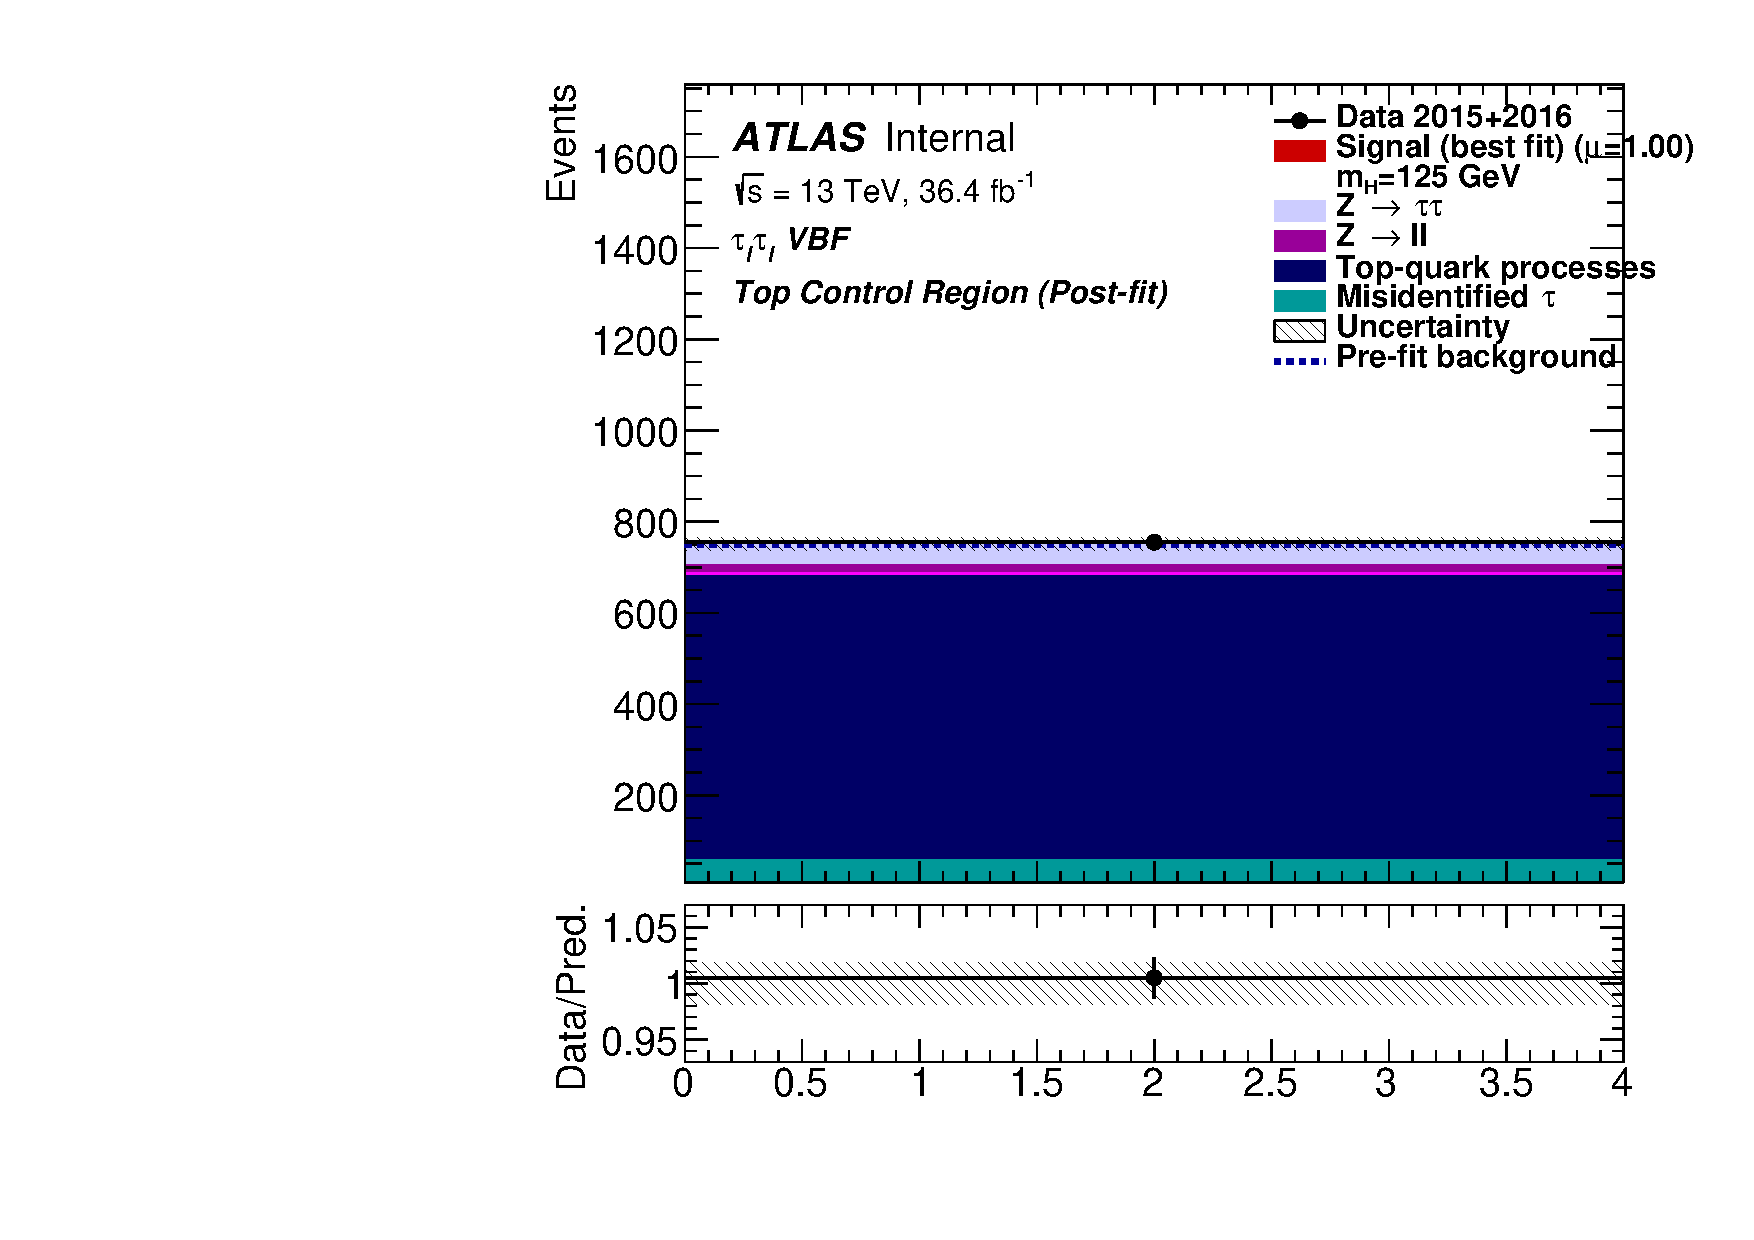
\includegraphics[width=\textwidth]{./plots/fit/mva/top_vbf.pdf}
        \caption{Top VBF}
    \end{subfigure}
    \caption{Distributions of the BDT output in the different control regions with the binning used in the fit of the multivariate analysis.
             For the data shown in the plot Asimov data corresponding to the 2015 and 2016 dataset with $\SI{36.1}{\invfb}$ are used.}\label{fig:fit:input:mva:CR}
\end{figure}

The expected significances for the cut-based and multivariate analysis are shown for fits in the individual signal regions
and for the combination of all signal regions in \cref{tab:fit:result:sigma}.
The multivariate analysis manages to increase the sensitivity by approximately \SI{33}{\percent} and \SI{72}{\percent} in the boosted and VBF category, respectively.
For the combined fit of the boosted and VBF category the increase is about \SI{63}{\percent}.

\begin{table}[htpb]
    \centering
    \caption{Expected significances for the cut-based (CBA) and multivariate (MVA) analysis of $\Httll$ for the combined and individual categories in units of $\sigma$.}\label{tab:fit:result:sigma}
    \begin{tabular}{lccccc}
        \toprule
        Analysis & Combined & Boosted & Boosted SF & Boosted DF & {VBF} \\ \midrule
        CBA      & 0.83     & 0.58    & --         & --         & 0.54  \\
        MVA      & 1.35     & 0.77    & 0.51       & 0.59       & 0.93  \\
        \bottomrule
    \end{tabular}
\end{table}

The results of the signal strength measurement in the cut-base and multivariate analysis are
\begin{align}
    \mu_\text{CBA} &= 1.0\, \errud{0.47}{0.46} \text{ (stat.) } \errud{1.25}{1.12} \text{ (sys.) }  \qquad \text{and} \\
    \mu_\text{MVA} &= 1.0\, \errud{0.32}{0.31} \text{ (stat.) } \errud{0.55}{0.66} \text{ (sys.) }  \,,
\end{align}
respectively.
Additionally, the results are visualized in \cref{fig:fit:result:mu}, where also the individual results for the VBF and boosted categories are shown.
Since Asimov data are used in the fit, the expected values are always 1.
However, it can be seen, that both the statistic and systematic uncertainties on the signal strengths are lower in the MVA than in the CBA\@.
The largest reduction of the uncertainties on the signal strength is in the VBF category, where the uncertainties decrease by a factor between 1.5 and 3.
The signal strength of the combined fit and measurement in the boosted category the uncertainties are reduced by a factor of up to two.


\begin{figure}[htb]
    \centering
    \begin{subfigure}[t]{0.45\textwidth}
        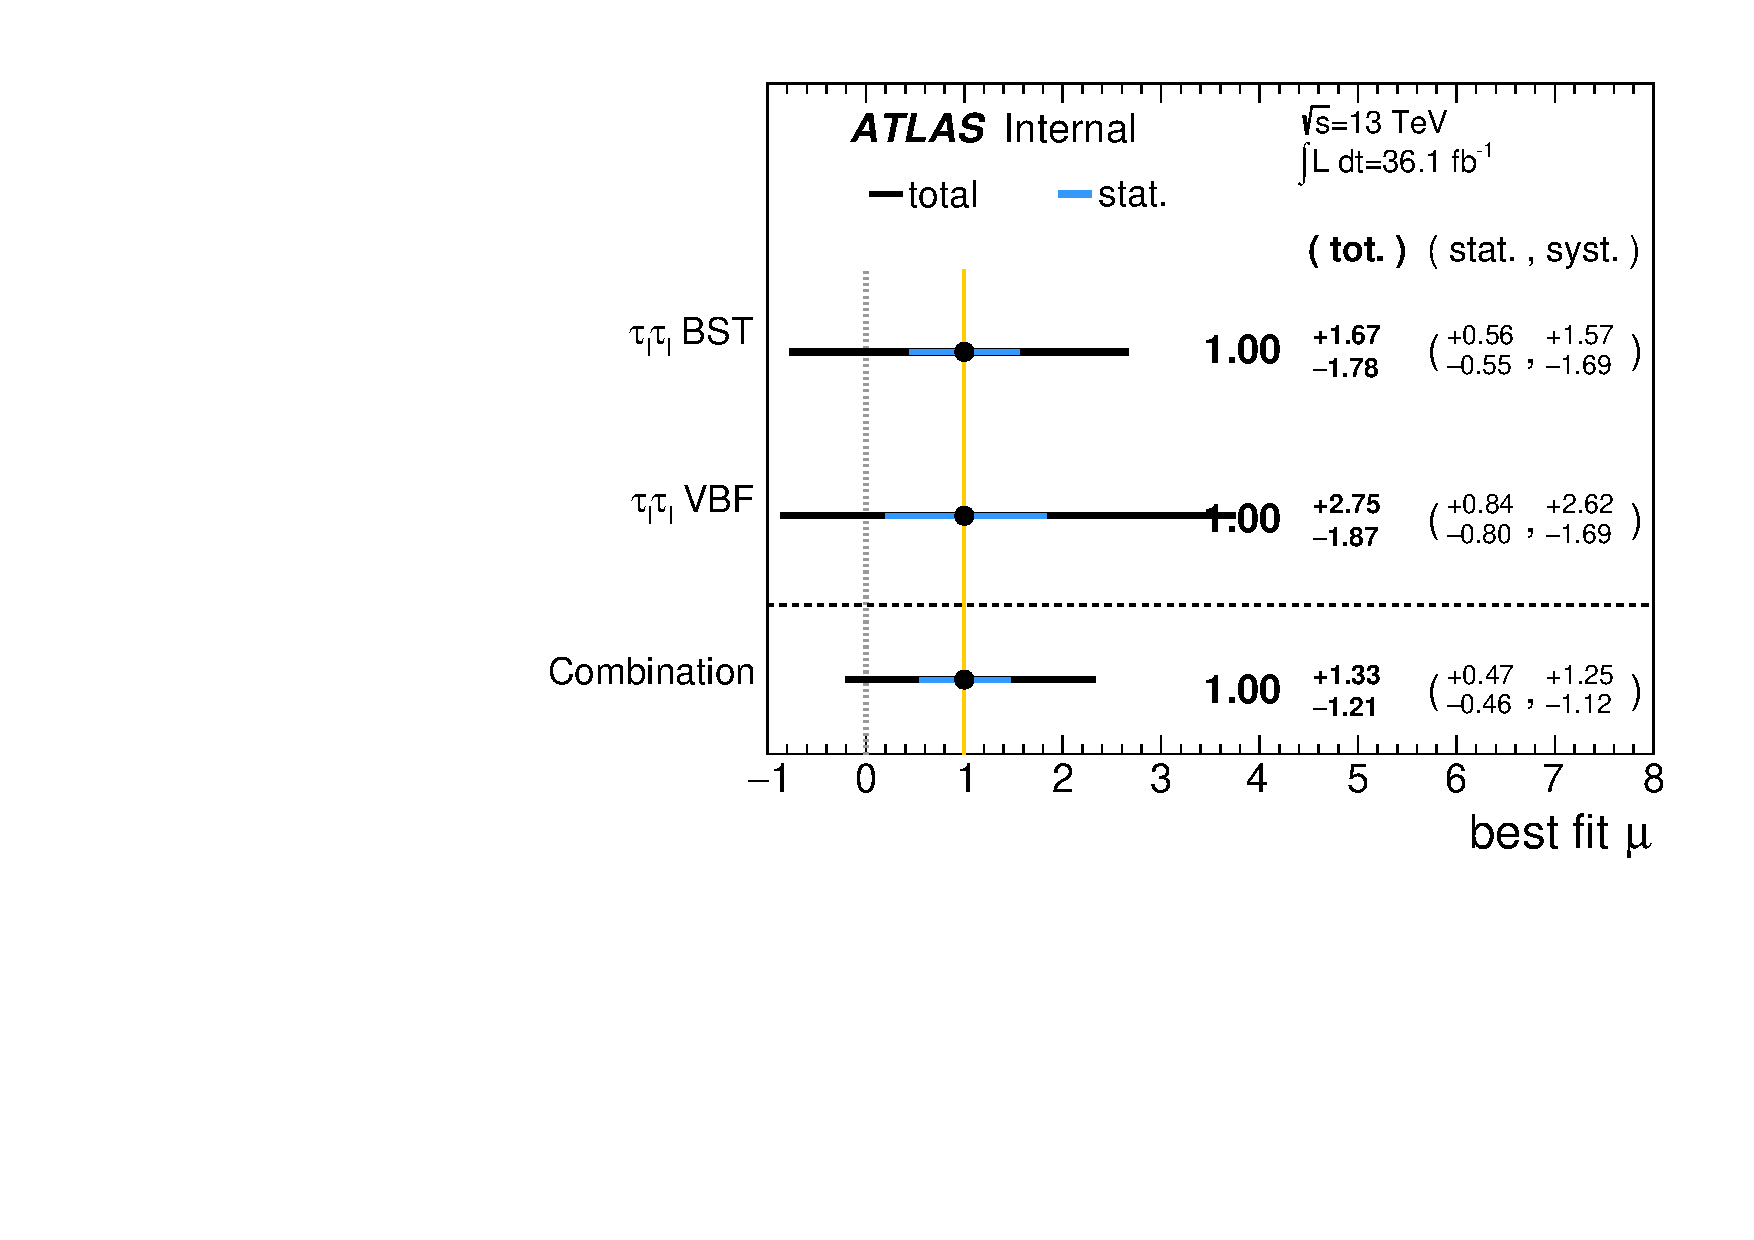
\includegraphics[width=\textwidth]{./plots/fit/cba/POI.pdf}
        \caption{CBA}
    \end{subfigure}
    \begin{subfigure}[t]{0.45\textwidth}
        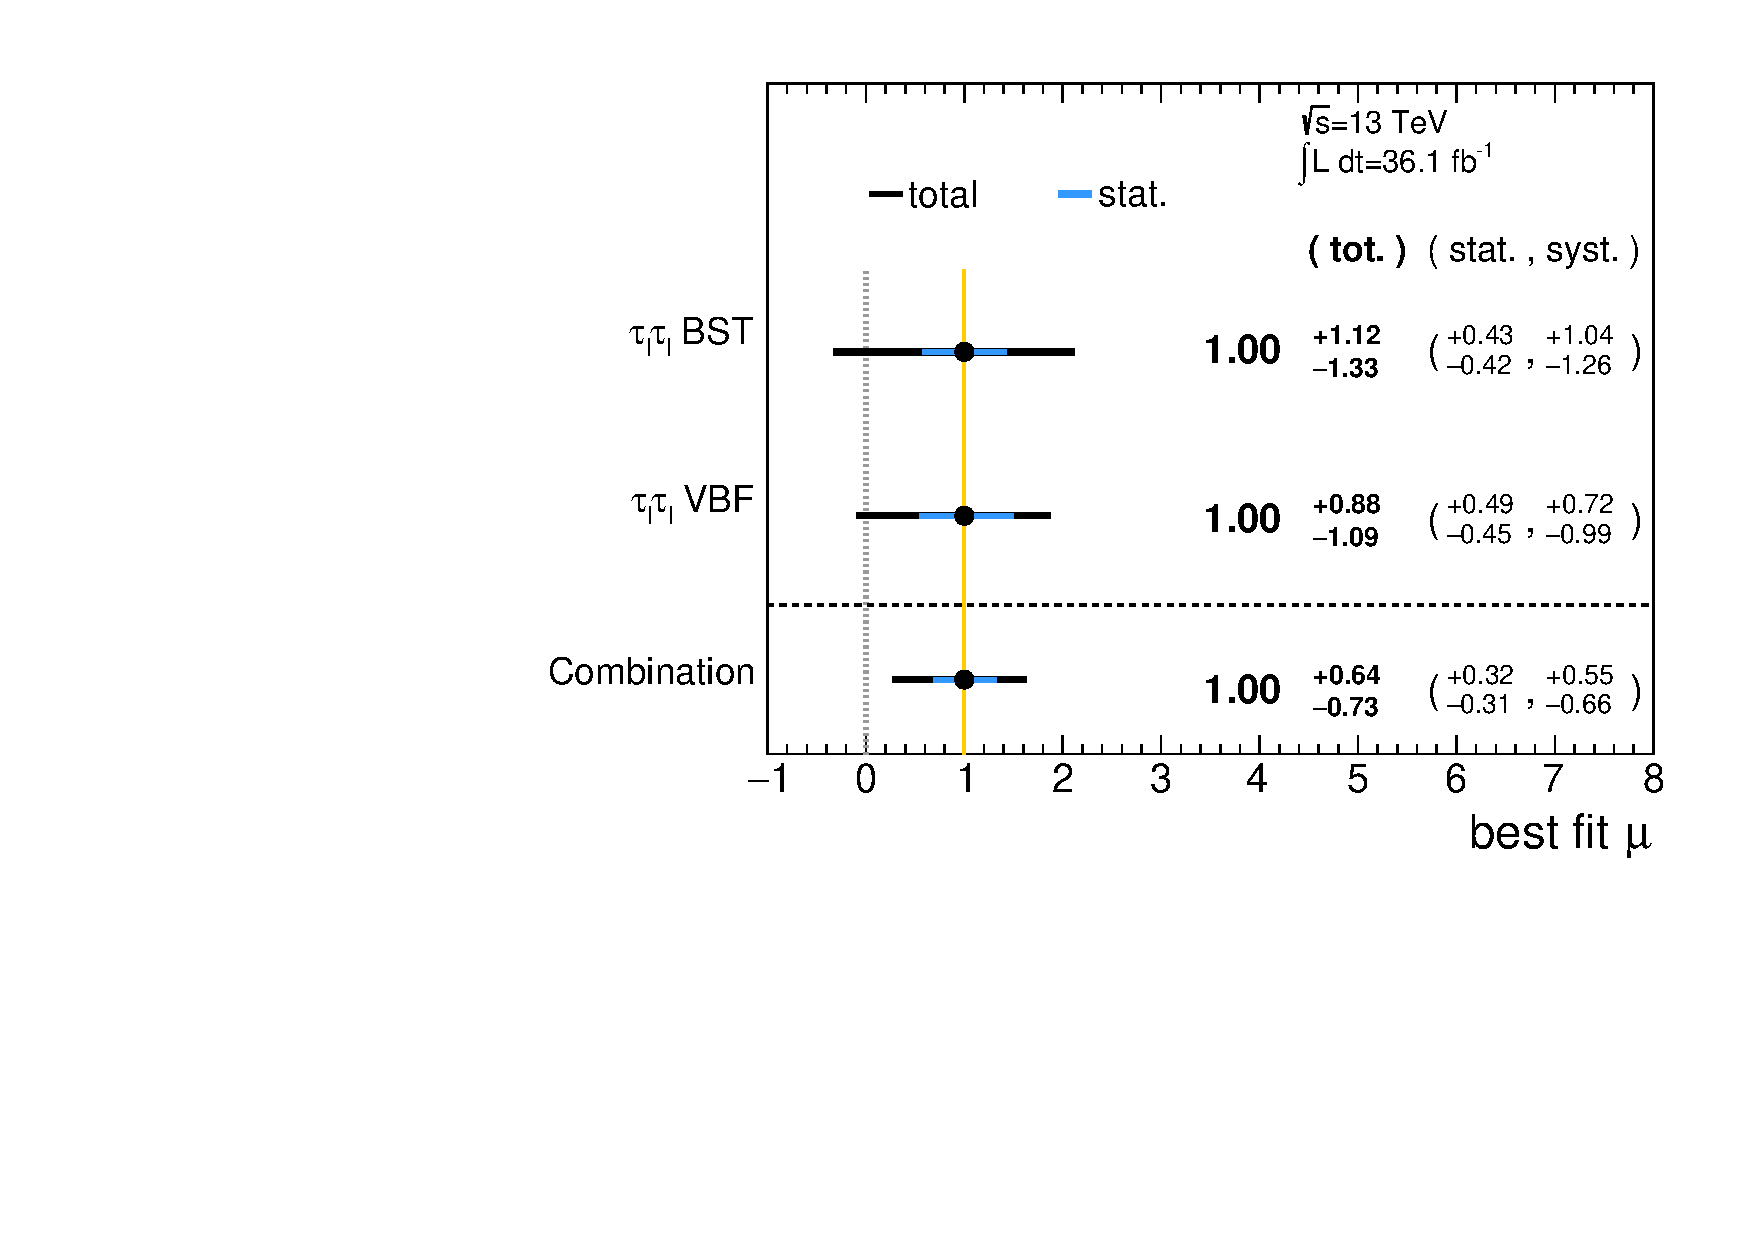
\includegraphics[width=\textwidth]{./plots/fit/mva/POI.pdf}
        \caption{MVA}
    \end{subfigure}
    \caption{Uncertainties on the signal strength measured in the cut-based analysis (a) and multivariate analysis (b)
             with Asimov data corresponding to the 2015 and 2016 dataset with $\SI{36.1}{\invfb}$.}\label{fig:fit:result:mu}
\end{figure}

A breakdown of the individual contributions to the uncertainties are given in \cref{tab:fit:result:uncert}.
The most dominate sources of uncertainty are related to measurements of jets and the missing transverse energy.
Furthermore, uncertainties due to count statistics in simulation and normalization of the $\Zll$, $\Ztautau$, and top-quark background
are also major sources of uncertainty.

\begin{table}[pb]
    \centering
    \caption{Uncertainty on the signal strength measurement in the cut-based (CBA) and multivariate (MVA) analysis
             with Asimov data corresponding to the 2015 and 2016 dataset with $\SI{36.1}{\invfb}$.}\label{tab:fit:result:uncert}
    \begin{tabular}{lcc}
        \toprule
         \multirow{2}{*}{Source of uncertainty} & \multicolumn{2}{c}{Impact on $\Delta \mu$ error}  \\
                                        & CBA        & MVA        \\ \midrule
         Total                          & $\pm 1.27$ & $\pm 0.68$ \\
         Data statistics                & $\pm 0.46$ & $\pm 0.32$ \\
         Systematic uncertainties       & $\pm 1.18$ & $\pm 0.60$ \\ \cmidrule{1-3}
         Normalization uncertainties    & $\pm 0.62$ & $\pm 0.25$ \\
         Jets and $\etmiss$             & $\pm 0.92$ & $\pm 0.45$ \\
         $b$-jets                       & $\pm 0.21$ & $\pm 0.03$ \\
         Light leptons                  & $\pm 0.12$ & $\pm 0.18$ \\
         Pileup reweighting             & $\pm 0.11$ & $\pm 0.04$ \\
         Fake estimation                & $\pm 0.17$ & $\pm 0.04$ \\
         Luminosity                     & $\pm 0.04$ & $\pm 0.04$ \\
         Theory unc.\ on signal         & $\pm 0.21$ & $\pm 0.09$ \\
         Theory unc.\ on $Z\to\tau\tau$ & $\pm 0.19$ & $\pm 0.07$ \\
         Simulation statistics          & $\pm 0.59$ & $\pm 0.32$ \\
         \bottomrule
    \end{tabular}
\end{table}
